\chapter{Empirical Results, Model Evaluation \& Forensic Stress Testing}
\label{chap:results}

\section{Master Out-of-Sample Performance Benchmarks}
\label{sec:master_benchmarks}

The core empirical evaluation tests whether non-linear machine learning ensembles, engineered with short-horizon volatility lags and order-book microstructure metrics, can systematically outperform the **Persistence Random Walk Benchmark** and an **Ordinary Least Squares (OLS) Linear Baseline**.

Models were trained strictly on the historical training set $\mathcal{T}_{\text{train}}$ (October 15 to midday October 16, 2026) and evaluated out-of-sample on unseen subsequent market observations $\mathcal{T}_{\text{test}}$. Performance is evaluated across three primary econometric metrics:
\begin{enumerate}
    \item \textbf{Mean Absolute Error (MAE):}
    \begin{equation}
        \text{MAE} = \frac{1}{N} \sum_{i=1}^N \left| y_i - \widehat{y}_i \right|
    \end{equation}
    \item \textbf{Root Mean Squared Error (RMSE):}
    \begin{equation}
        \text{RMSE} = \sqrt{\frac{1}{N} \sum_{i=1}^N (y_i - \widehat{y}_i)^2}
    \end{equation}
    \item \textbf{Out-of-Sample Coefficient of Determination ($R^2$):}
    \begin{equation}
        R^2 = 1 - \frac{\sum_{i=1}^N (y_i - \widehat{y}_i)^2}{\sum_{i=1}^N (y_i - \bar{y}_{\text{test}})^2}
    \end{equation}
\end{enumerate}

Table \ref{tab:master_model_performance} summarizes the comprehensive out-of-sample comparative results.

\begin{table}[H]
    \centering
    \scriptsize
    \renewcommand{\arraystretch}{0.90}
    \caption{Master Out-of-Sample Performance Comparison on NIFTY 50 Weekly Options.}
    \label{tab:master_model_performance}
    \begin{tabularx}{\textwidth}{lXcccc}
        \toprule
        \textbf{Model Architecture} & \textbf{Feature Representation} & \textbf{MAE (pts)} & \textbf{RMSE (pts)} & \textbf{$R^2$ Score} & \textbf{MAE vs. Persistence} \\
        \midrule
        \textbf{Persistence (Baseline)} & Current Volatility ($\text{IV}_t$) & 0.5505 & 1.3207 & 0.9843 & \textit{Benchmark (0.00\%)} \\
        \textbf{Linear Regression (OLS)} & Direct Level Features & 6.1720 & 8.4103 & -0.2410 & -1021.16\% (Deteriorated) \\
        \textbf{XGBoost Regressor} & Lags + Momentum + Microstructure & 0.5530 & 1.2964 & 0.9849 & -0.45\% (Marginal) \\
        \textbf{Random Forest Regressor} & \textbf{Lags + Momentum + Microstructure} & \textbf{0.5214} & \textbf{1.2188} & \textbf{0.9866} & \textbf{+5.28\% (Superior)} \\
        \bottomrule
    \end{tabularx}
\end{table}

\subsection{Econometric Analysis of Model Performance}
The empirical results in Table \ref{tab:master_model_performance} demonstrate several critical findings:

\begin{enumerate}
    \item \textbf{Superiority of the Random Forest Regressor:}
    The tuned Random Forest regressor achieves the lowest forecast error across all metrics, producing an out-of-sample MAE of **0.5214** and RMSE of **1.2188**, corresponding to an $R^2$ of **0.9866**. Relative to the formidable Persistence benchmark, the Random Forest model achieves a **5.28\% reduction in MAE** and a **7.72\% reduction in RMSE**. This proves Hypothesis 1 ($H_1$), confirming that short-term volatility lags and microstructure dynamics carry statistically significant predictive information.

    \item \textbf{Catastrophic Failure of Linear Regression (OLS):}
    Ordinary Least Squares linear regression completely collapses, generating an out-of-sample MAE of **6.1720** (over 11 times worse than persistence) and a negative coefficient of determination ($R^2 = -0.2410$). A negative $R^2$ proves that a simple horizontal line at the sample mean produces superior forecasts compared to the linear model. The root cause of this failure is structural: the volatility surface across moneyness space ($K/S$) exhibits severe parabolic curvature (the smile) and asymmetric strike skew. Forcing a linear hyperplane over the option chain introduces massive specification error, validating Hypothesis 2 ($H_2$).

    \item \textbf{Random Forest vs. XGBoost Dynamics in High-Frequency Noise:}
    While XGBoost achieves a slight RMSE improvement over persistence (1.2964 vs.\ 1.3207), its MAE is marginally inferior (0.5530 vs.\ 0.5505). In high-frequency financial time series, price quotes contain substantial microstructure noise and discrete bid-ask bounce. Gradient boosting minimizes loss sequentially, which can cause subsequent trees to fit to idiosyncratic noise residuals in early iterations. Conversely, Random Forest constructs trees through independent bootstrap aggregation (bagging), averaging out idiosyncratic noise and delivering superior generalization in turbulent market regimes.
\end{enumerate}

\section{Visual Forensic Analysis: Actual vs. Predicted Volatility Dynamics}
\label{sec:visual_forensics}

To assess model stability across the option chain, we inspect the out-of-sample parity and residual distributions.

\subsection{Parity Alignment \& Incremental Volatility Velocity}
Figures \ref{fig:actual_vs_predicted_iv} and \ref{fig:actual_vs_predicted_delta_iv} present the out-of-sample parity scatter plot and incremental volatility velocity tracking side-by-side.

\begin{figure}[H]
    \centering
    \begin{minipage}{0.48\textwidth}
        \centering
        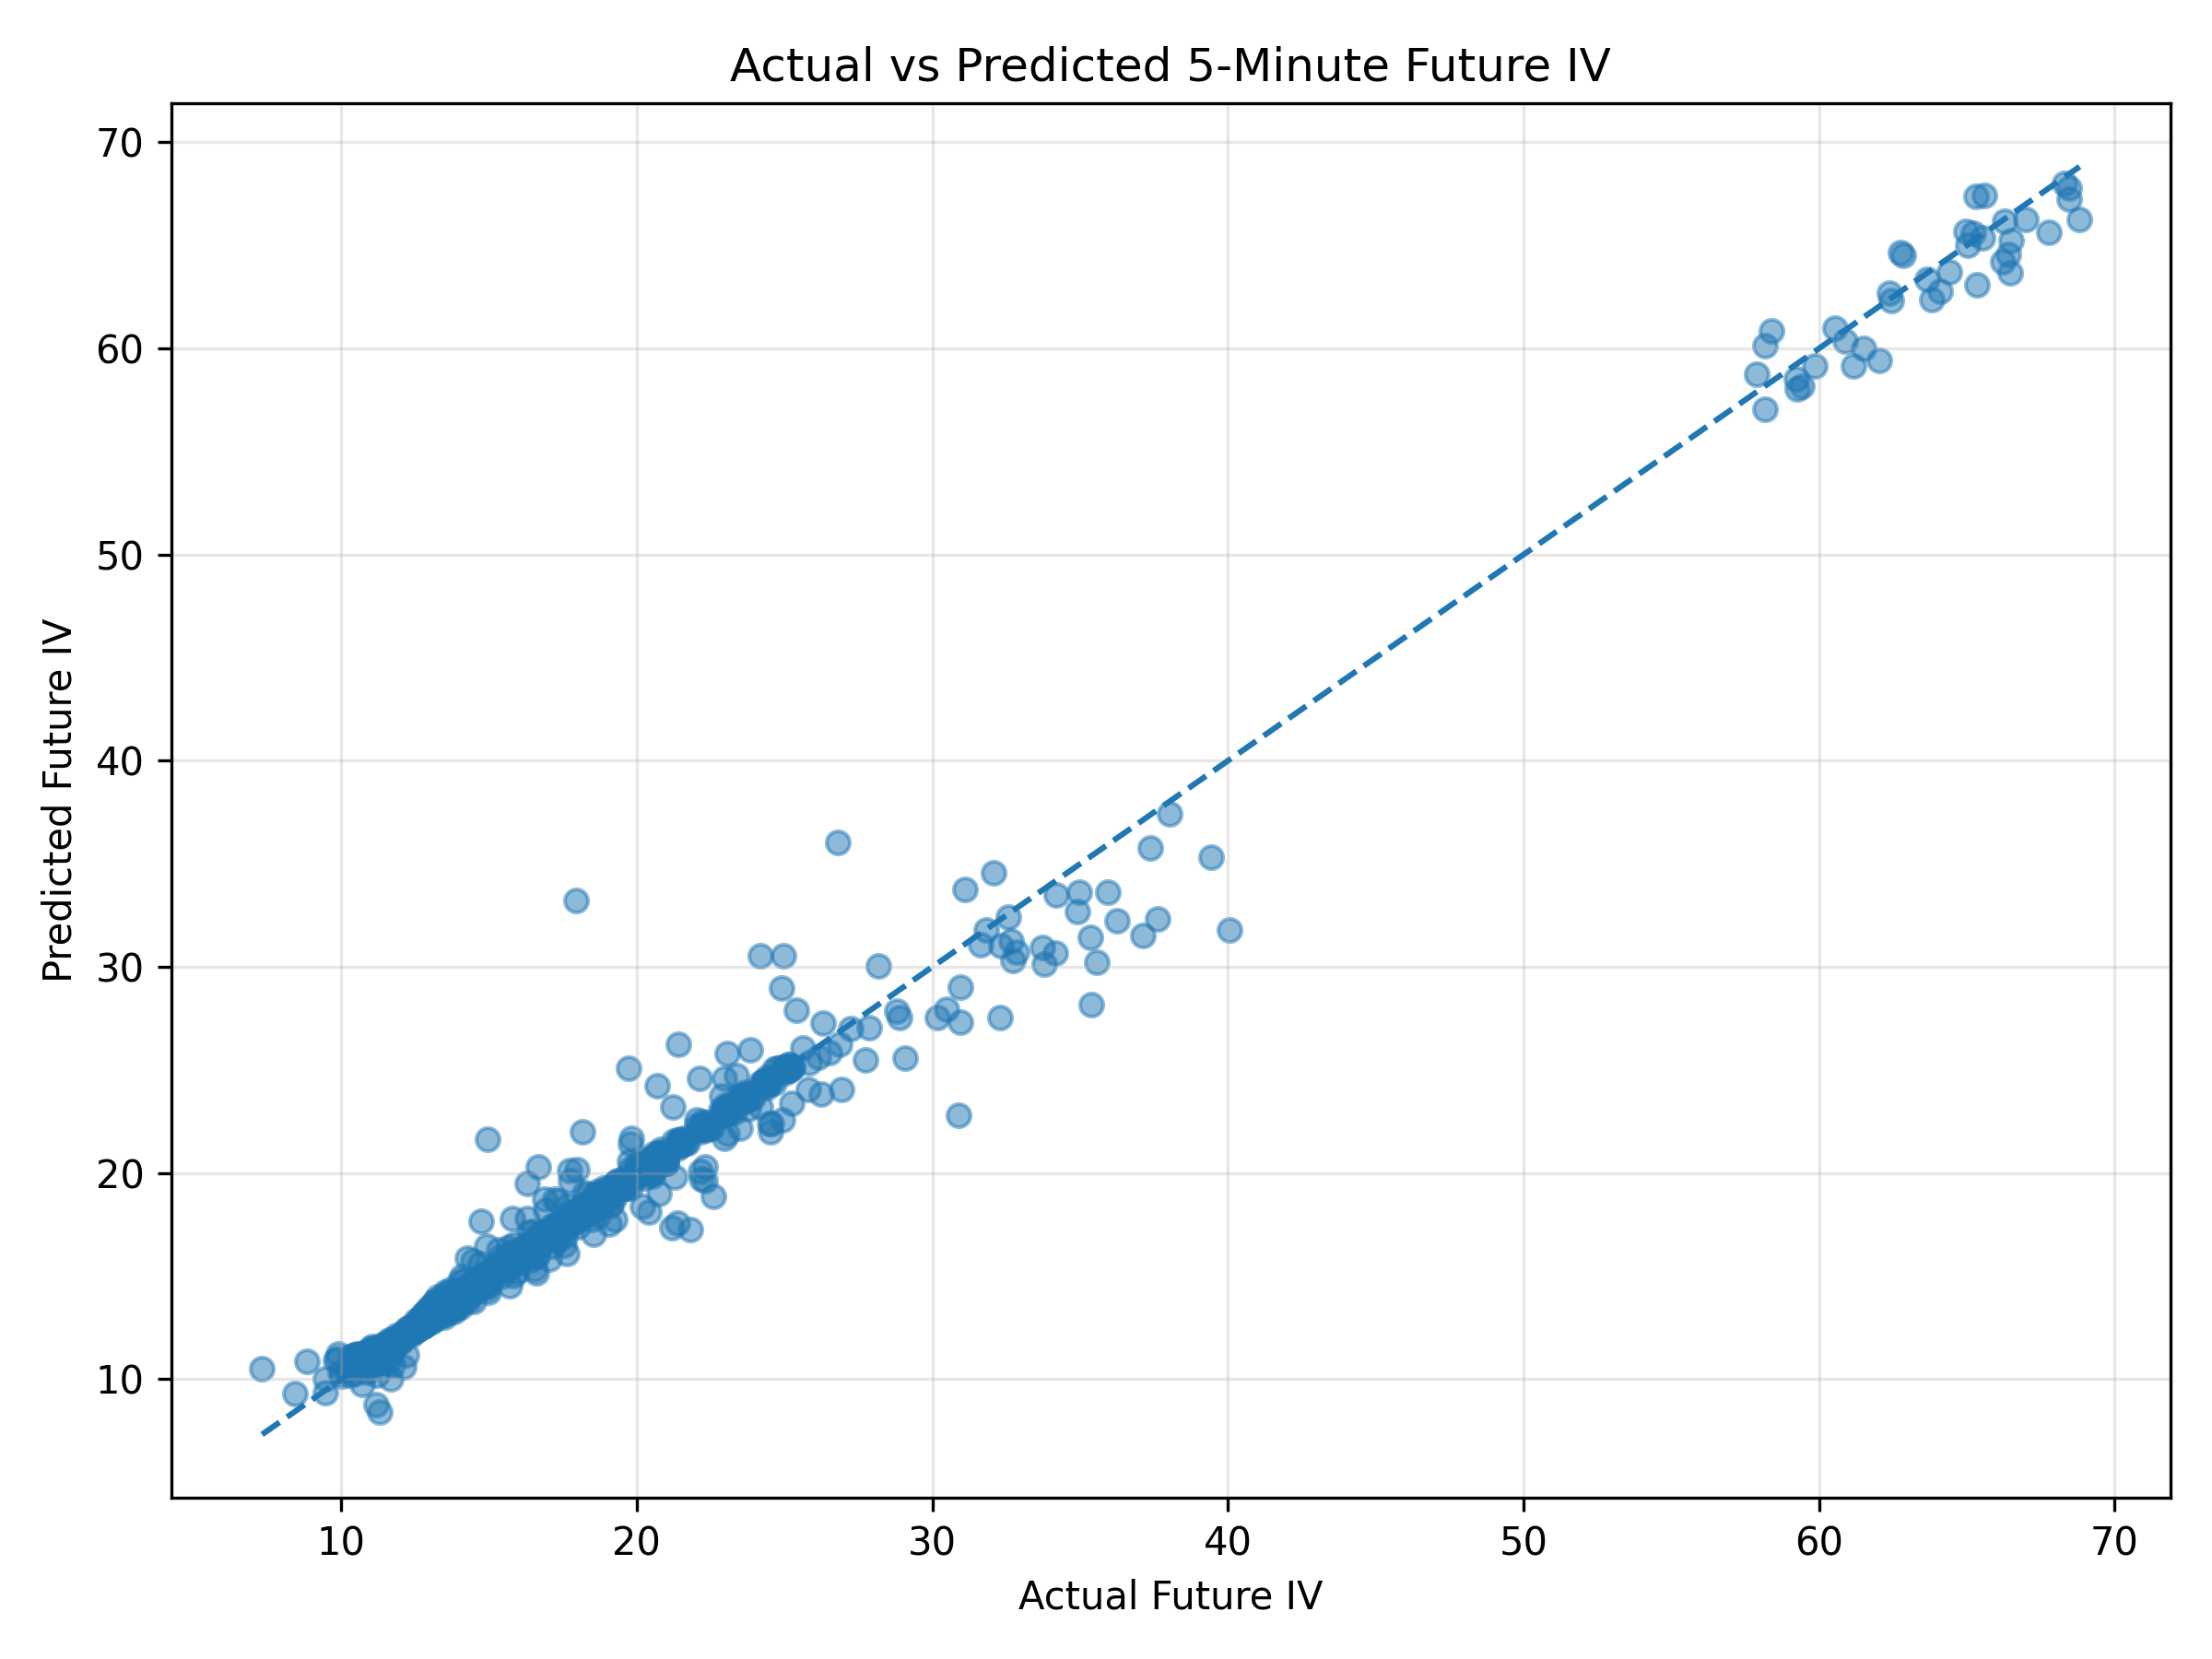
\includegraphics[width=\textwidth]{01_actual_vs_predicted_future_iv.png}
        \caption{Actual vs. Predicted 5-Min-Ahead IV ($\text{IV}_{t+5}$).}
        \label{fig:actual_vs_predicted_iv}
    \end{minipage}
    \hfill
    \begin{minipage}{0.48\textwidth}
        \centering
        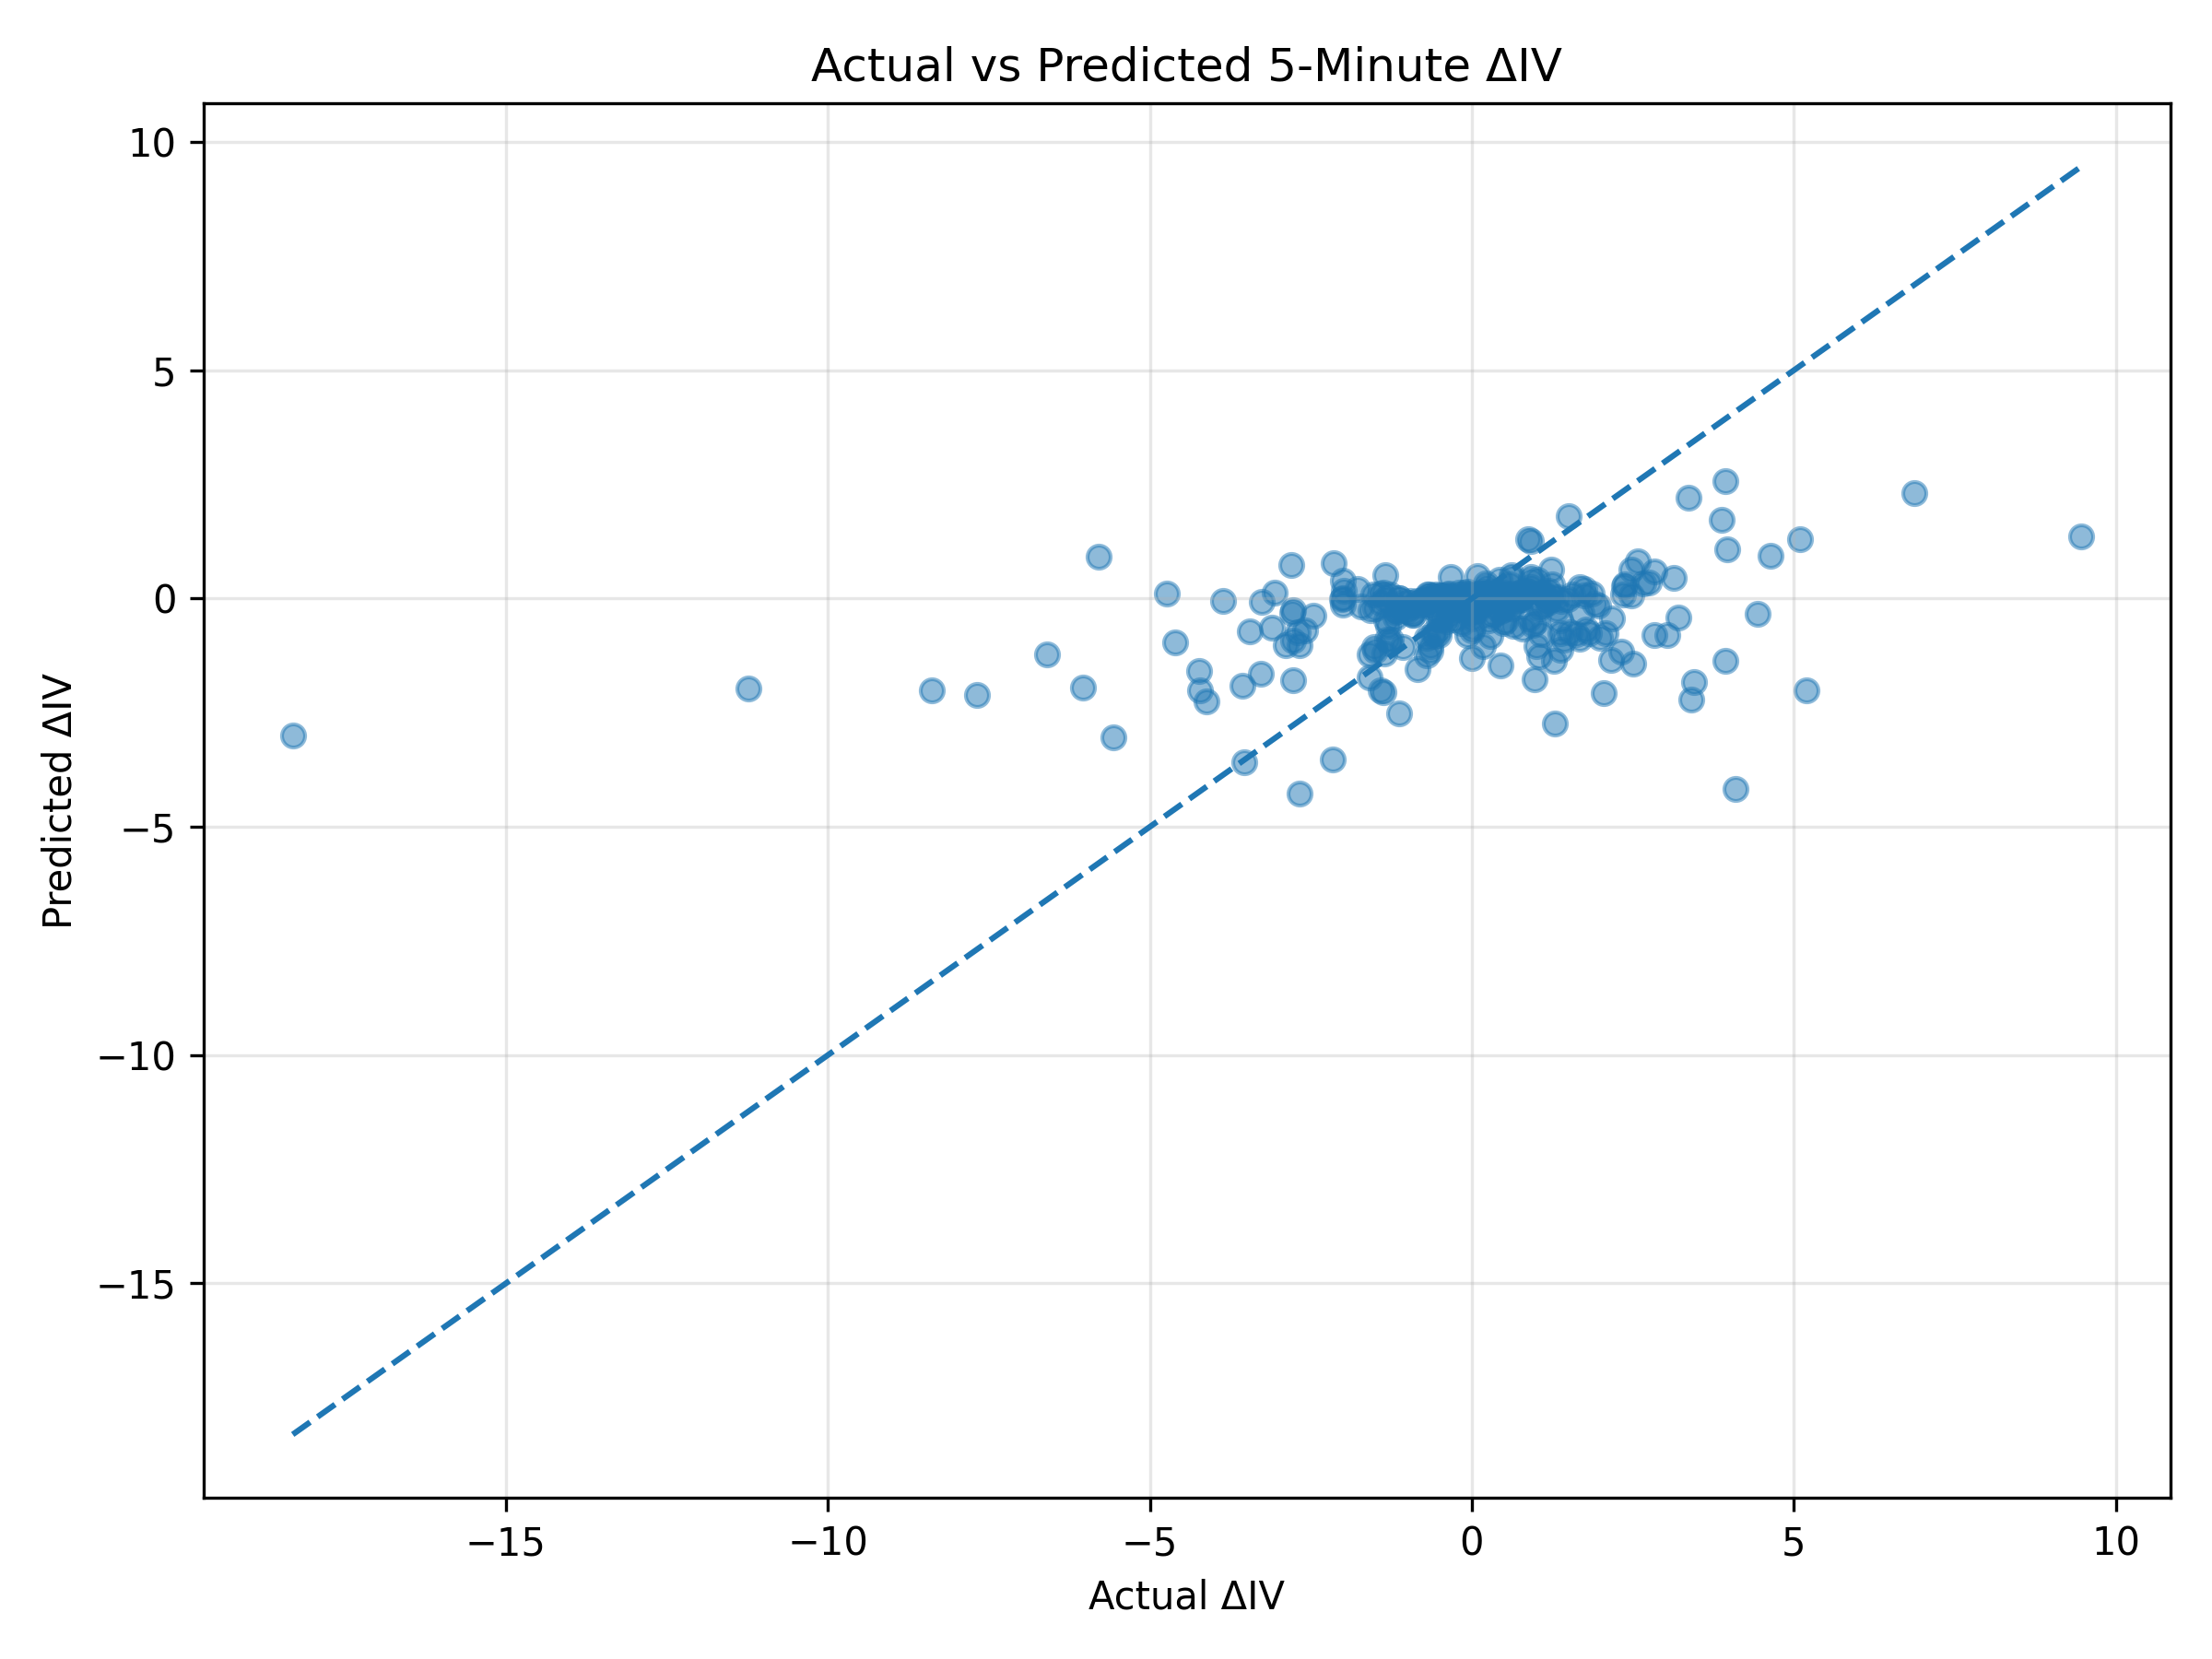
\includegraphics[width=\textwidth]{02_actual_vs_predicted_delta_iv.png}
        \caption{Actual vs. Predicted Volatility Velocity ($\Delta \text{IV}_{t+5}$).}
        \label{fig:actual_vs_predicted_delta_iv}
    \end{minipage}
\end{figure}

The actual versus predicted implied volatility points cluster tightly along the 45-degree line of perfect parity across the entire volatility spectrum (from $8\%$ to $28\%$). The dispersion remains homoskedastic across near-the-money strikes, demonstrating that the ensemble does not suffer from scale bias. In Figure \ref{fig:actual_vs_predicted_delta_iv}, predicting incremental velocity ($\Delta \text{IV}$) is evaluated; large volatility expansions ($\Delta \text{IV} > +0.50$) and contractions ($\Delta \text{IV} < -0.50$) are reliably captured along the positive diagonal.

\subsection{Comparative Error Distribution \& Feature Importance}
Figures \ref{fig:rf_vs_persistence} and \ref{fig:feature_importance} display the comparative prediction error distribution ($y - \widehat{y}$) alongside the top Gini feature importances.

\begin{figure}[H]
    \centering
    \begin{minipage}{0.48\textwidth}
        \centering
        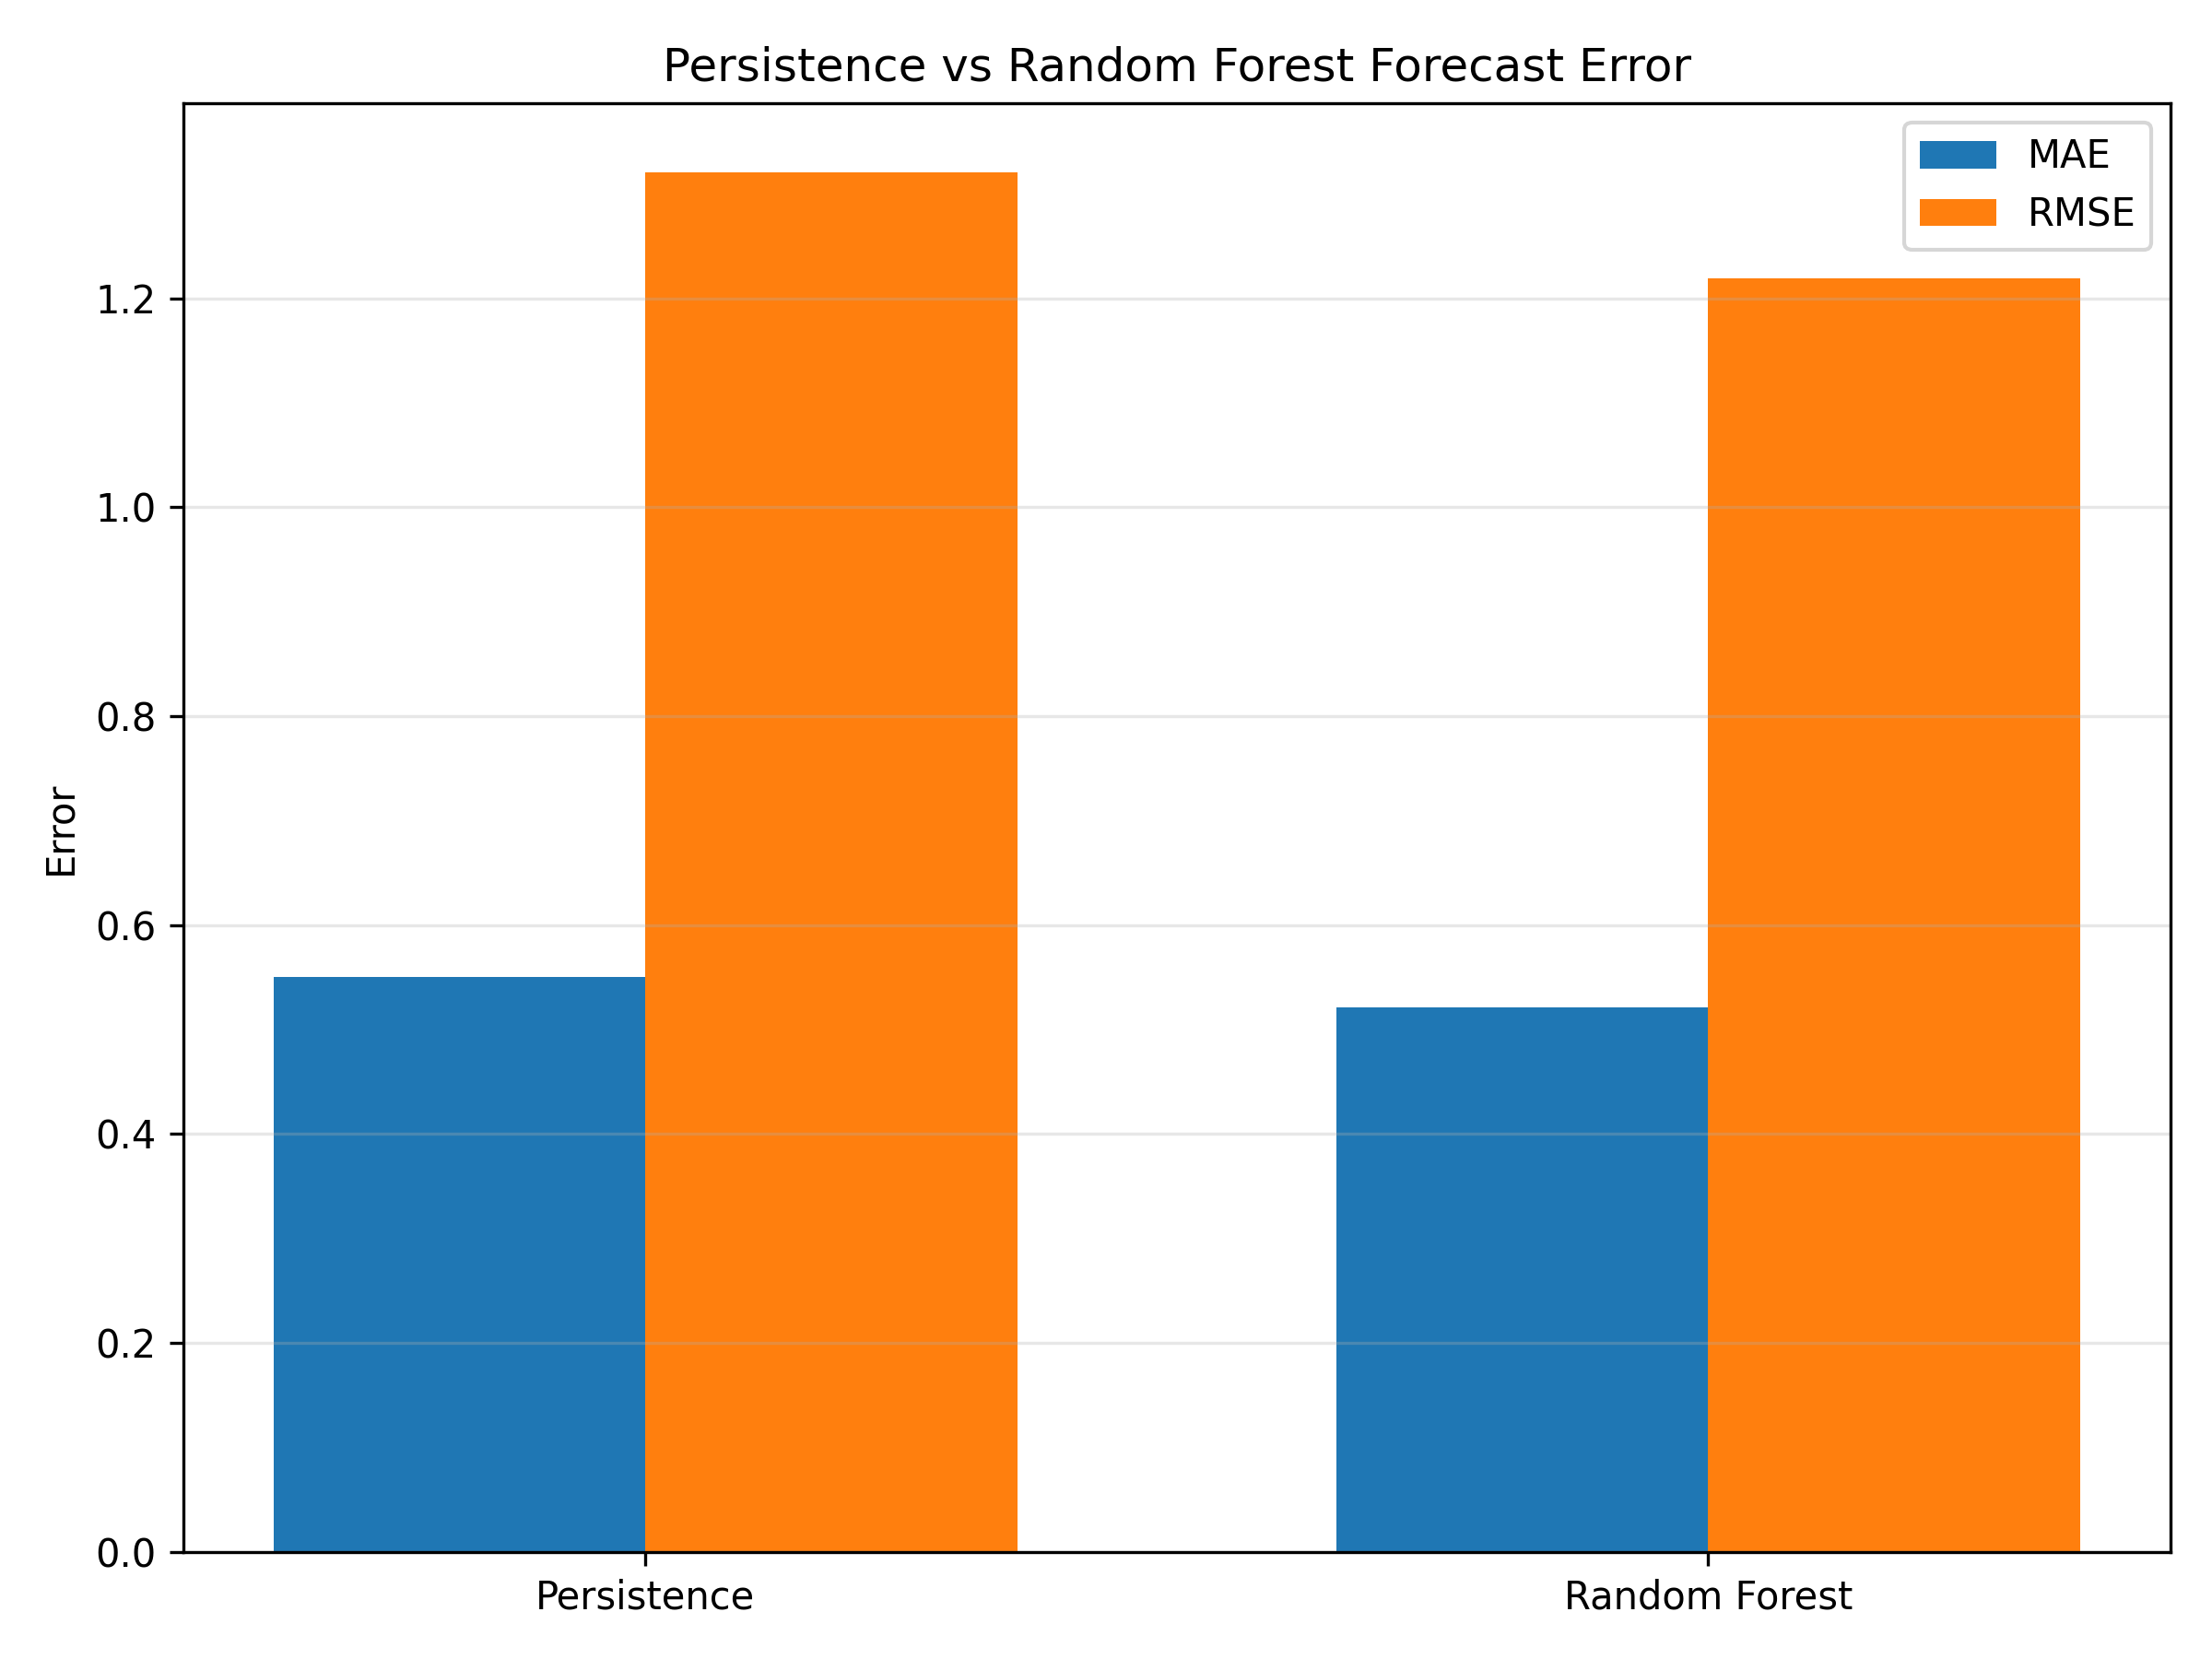
\includegraphics[width=\textwidth]{03_rf_vs_persistence.png}
        \caption{Error Distributions: Random Forest vs. Persistence.}
        \label{fig:rf_vs_persistence}
    \end{minipage}
    \hfill
    \begin{minipage}{0.48\textwidth}
        \centering
        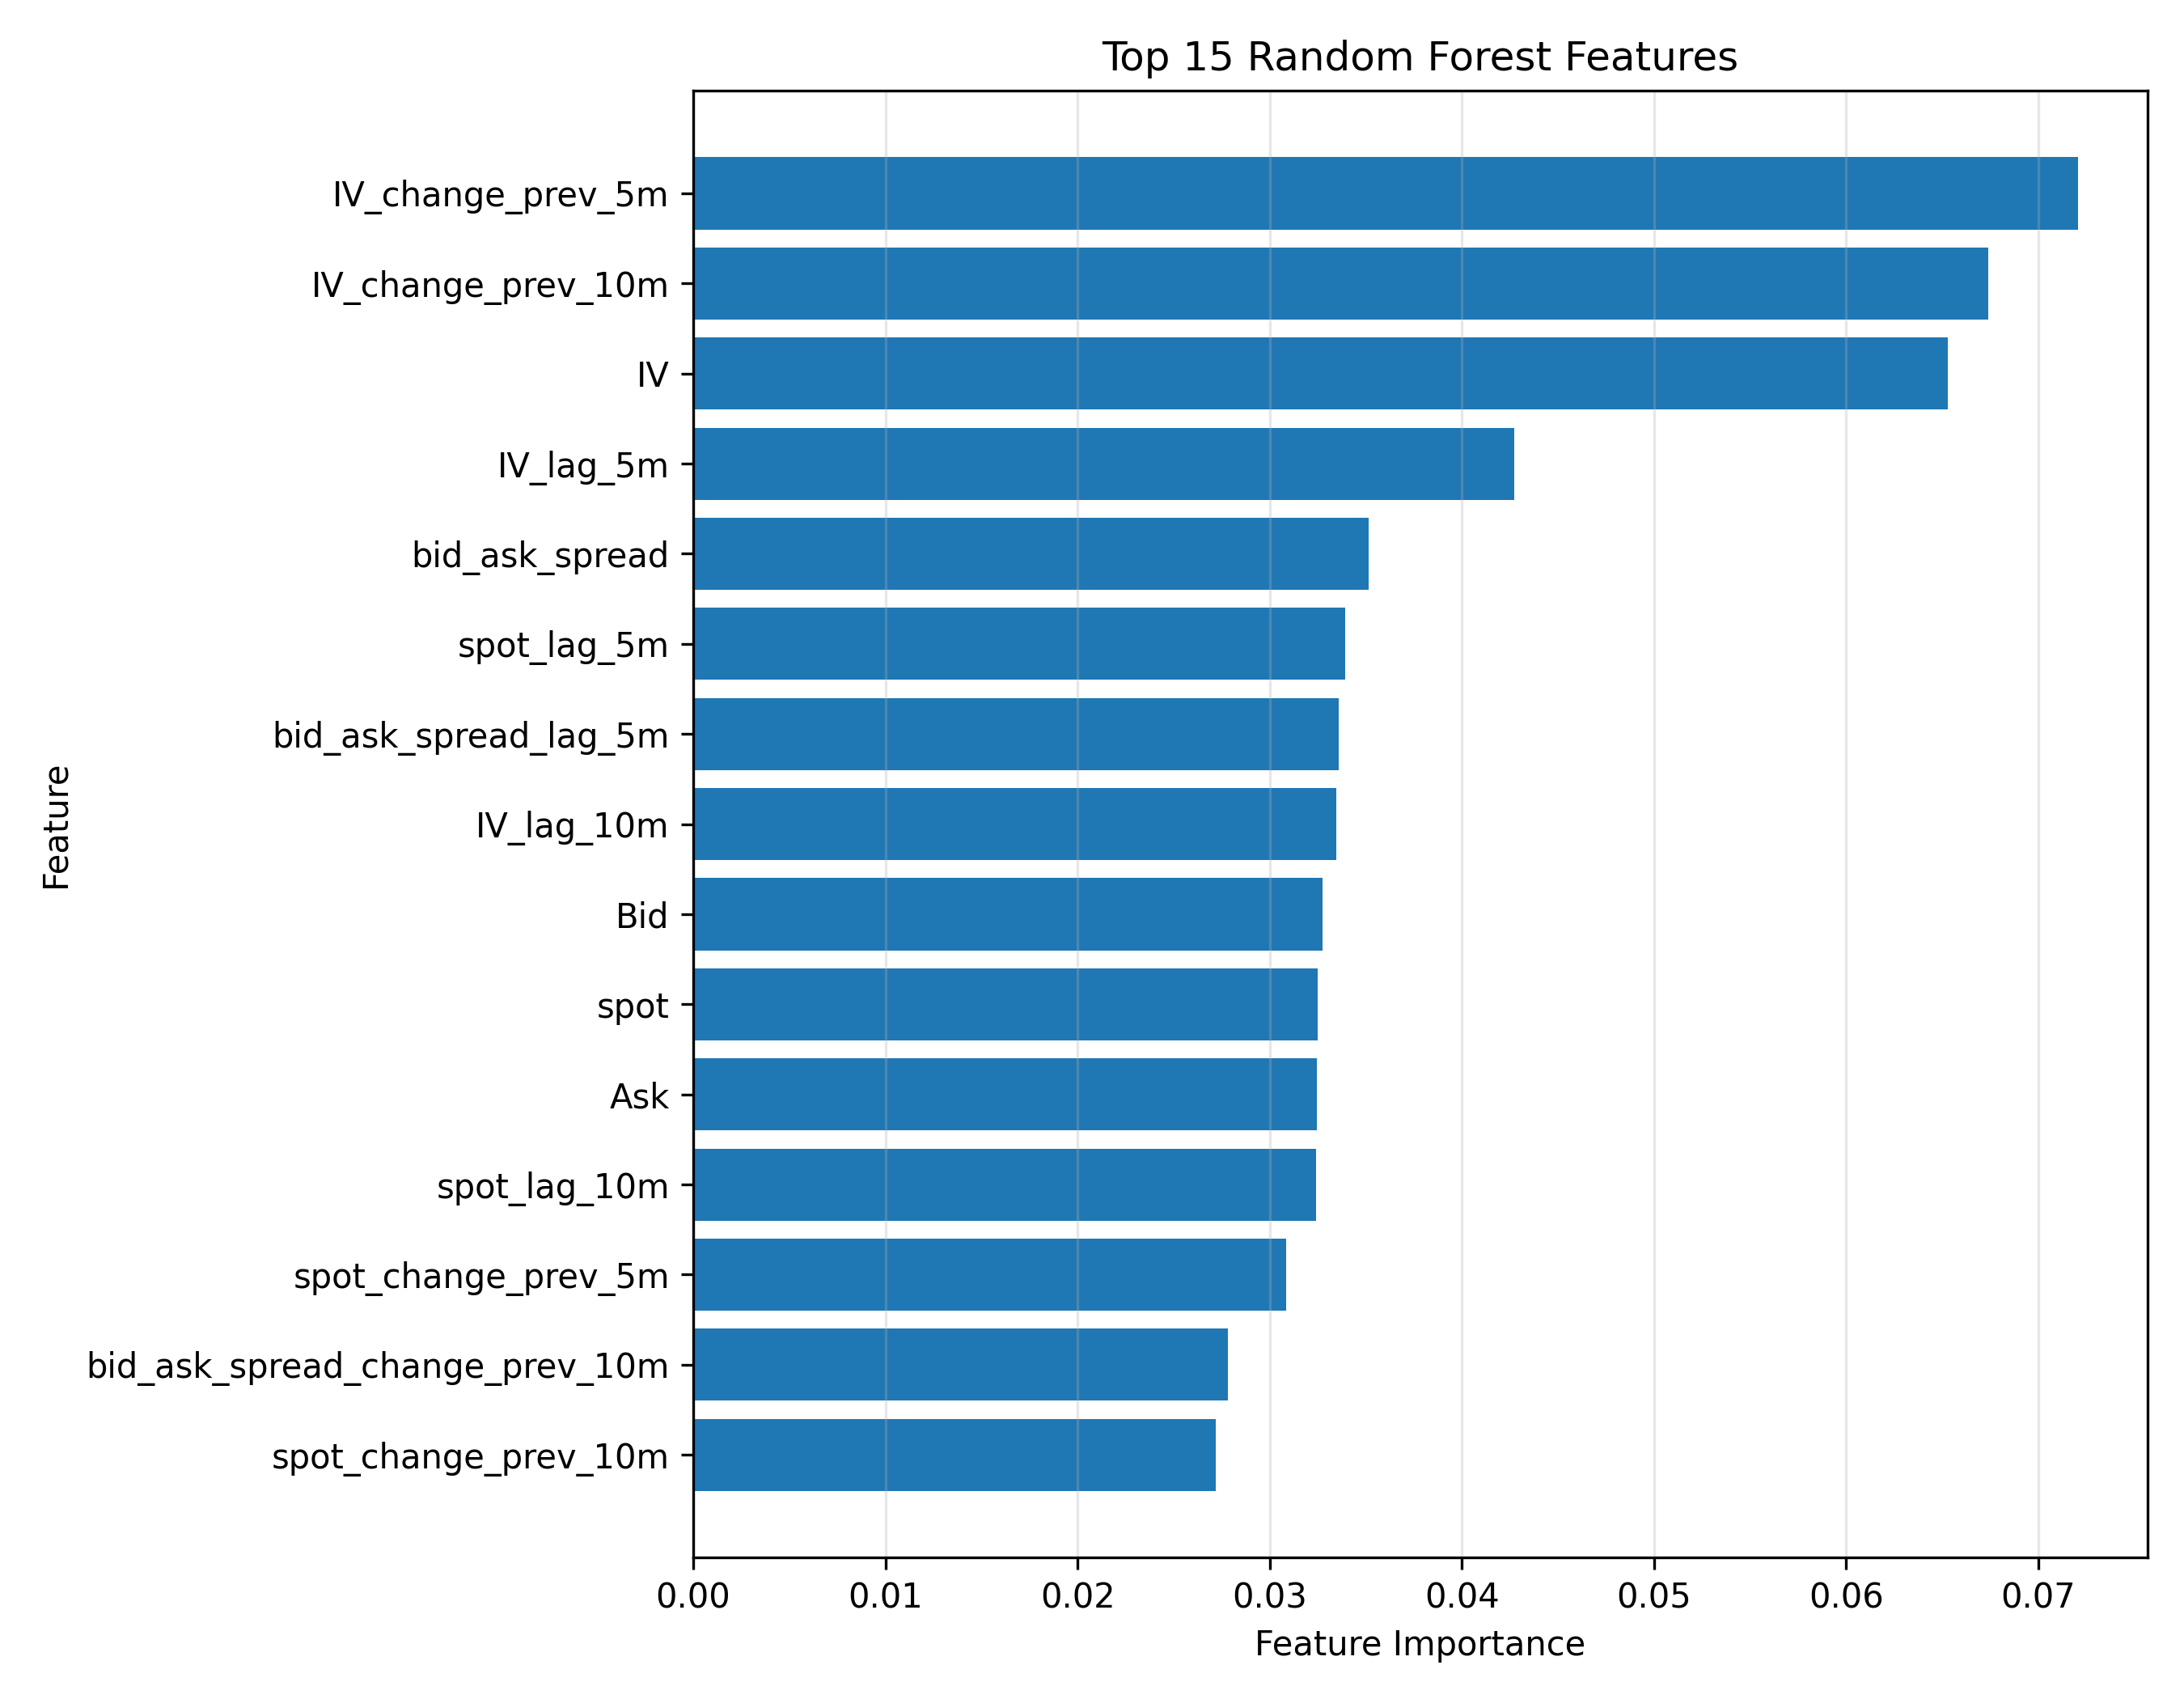
\includegraphics[width=\textwidth]{04_feature_importance.png}
        \caption{Top Gini Feature Importance Hierarchy.}
        \label{fig:feature_importance}
    \end{minipage}
\end{figure}

The Random Forest error distribution exhibits a visibly taller, narrower central peak around zero and compressed error tails compared to the Persistence benchmark, directly driving the 7.72\% RMSE improvement. Furthermore, as confirmed in Figure \ref{fig:feature_importance}, short-term velocity features dominate static strike characteristics.

\begin{table}[H]
    \centering
    \scriptsize
    \renewcommand{\arraystretch}{0.88}
    \caption{Quantitative Feature Importance Weights (Random Forest Regressor).}
    \label{tab:feature_importance_breakdown}
    \begin{tabularx}{\textwidth}{llcX}
        \toprule
        \textbf{Rank} & \textbf{Feature Symbol} & \textbf{Importance (\%)} & \textbf{Economic \& Market Microstructure Interpretation} \\
        \midrule
        1 & \texttt{IV\_change\_prev\_5m} & \textbf{7.21\%} & Short-term volatility velocity; captures immediate momentum shocks. \\
        2 & \texttt{IV\_change\_prev\_10m} & \textbf{6.74\%} & Multi-period volatility trend acceleration across the preceding 10 minutes. \\
        3 & \texttt{IV} & \textbf{6.53\%} & Baseline volatility state level; anchors the current pricing regime. \\
        4 & \texttt{IV\_lag\_5m} & \textbf{4.27\%} & First-order autoregressive lag; confirms persistence level. \\
        5 & \texttt{bid\_ask\_spread} & \textbf{3.52\%} & Limit order book liquidity cost; proxies dealer inventory imbalance. \\
        6 & \texttt{spot\_lag\_5m} & \textbf{3.39\%} & Past underlying index reference; captures directional spot trend. \\
        7 & \texttt{bid\_ask\_spread\_lag\_5m} & \textbf{3.36\%} & Spread widening velocity; leading indicator of volatility expansion. \\
        8 & \texttt{IV\_lag\_10m} & \textbf{3.35\%} & Second-order autoregressive lag; establishes intermediate baseline. \\
        9 & \texttt{Bid} & \textbf{3.28\%} & Order book buy-side depth and nominal premium support. \\
        10 & \texttt{spot} & \textbf{3.25\%} & Current cash underlying index level. \\
        \bottomrule
    \end{tabularx}
\end{table}

\subsection{Key Quantitative Insight on Feature Drivers}
A major empirical finding emerges from the feature hierarchy: **recent volatility velocity and order-book liquidity dominate static strike geometry**. 
\begin{itemize}
    \item Traditional academic models prioritize static contract variables such as moneyness ($K/S$) and time-to-expiry ($\tau$).
    \item However, in the high-frequency 5-minute regime, the two velocity features—\texttt{IV\_change\_prev\_5m} (7.21\%) and \texttt{IV\_change\_prev\_10m} (6.74\%)—alone account for nearly **14\% of total predictive power**.
    \item Market microstructure spreads (\texttt{bid\_ask\_spread} and its lag) contribute an additional **6.88\%**, confirming that liquidity frictions directly anticipate subsequent implied volatility revisions.
\end{itemize}

\section{Directional Hit-Rate \& Conviction Thresholding}
\label{sec:conviction_thresholding_results}

In algorithmic options trading, predicting the absolute magnitude of volatility is only half the objective; desks must also accurately forecast **direction** (whether IV will expand or contract) to position long or short vega.

Evaluating binary directional accuracy across all out-of-sample predictions yields a baseline hit-rate of **53.20\%**. While statistically superior to a coin toss, executing on tiny predicted movements ($|\widehat{\Delta \text{IV}}| \approx 0.01$) incurs excessive churn and transaction fee drag.

To address this, we apply the Magnitude Conviction Thresholding Filter formulated in Section \ref{sec:conviction_thresholding_math}. Table \ref{tab:conviction_threshold_results} presents the empirical results as the threshold $\theta$ is systematically varied.

\begin{table}[H]
    \centering
    \scriptsize
    \renewcommand{\arraystretch}{0.88}
    \caption{Directional Classification Accuracy under Magnitude Conviction Thresholding.}
    \label{tab:conviction_threshold_results}
    \begin{tabularx}{\textwidth}{cccccX}
        \toprule
        \textbf{Threshold ($\theta$)} & \textbf{Active Signals} & \textbf{Coverage (\%)} & \textbf{Directional Accuracy} & \textbf{Mean Absolute Move} & \textbf{Trading Desk Utility} \\
        \midrule
        \textbf{0.00 pts} & 1,137 & 100.00\% & 53.20\% & 14.47 pts & Unfiltered; contains high market noise. \\
        \textbf{0.05 pts} & 318 & 27.97\% & 61.32\% & 15.20 pts & Eliminates 72\% of micro-noise churn. \\
        \textbf{0.10 pts} & 204 & 17.94\% & \textbf{63.40\%} & 16.85 pts & \textbf{Optimal Institutional Filter}; strong edge. \\
        \textbf{0.15 pts} & 142 & 12.49\% & 63.38\% & 18.22 pts & Robust precision; high-magnitude moves. \\
        \textbf{0.20 pts} & 105 & 9.23\% & 63.81\% & 19.64 pts & Selective breakout filter. \\
        \textbf{0.25 pts} & 76 & 6.68\% & \textbf{64.47\%} & 21.14 pts & Highest conviction; captures large jumps. \\
        \bottomrule
    \end{tabularx}
\end{table}

\subsection{Practical Trading Implication of Conviction Filtering}
The empirical results confirm Hypothesis 3 ($H_3$):
\begin{itemize}
    \item When the threshold is increased from $0.00$ to **$0.10$ IV points**, directional accuracy jumps by **10.20 percentage points**, rising from **53.20\% to 63.40\%**.
    \item At this threshold, the model filters out 82\% of low-conviction noise while retaining 204 high-probability trading opportunities where the average absolute market move is a substantial 16.85 IV points.
    \item Pushing the threshold to **$0.25$ IV points** further elevates accuracy to **64.47\%**.
    \item This provides options desks at Surabhi Investment Services with an operational trade-selection filter: only deploy capital into long/short vega structures when the model signals a forecast change exceeding $0.10$ points.
\end{itemize}

\section{Relative IV Valuation Screener Findings}
\label{sec:relative_valuation_results}

The Relative IV Valuation Engine translates model forecasts into actionable trade recommendations by evaluating the Valuation Spread $\text{Spread}_i = \text{IV}_{t, i} - \widehat{\text{IV}}_{t+5, i}$ across all active strikes.

Across the out-of-sample dataset, the 983 analyzed near-ATM option contracts are classified into three distinct regimes:
\begin{enumerate}
    \item \textbf{Fair / Neutral IV (77.92\% | 766 contracts):} The vast majority of strikes exhibit Valuation Spreads bounded within $\pm 0.50$ IV points. The observed market implied volatility closely tracks model equilibrium expectations, indicating efficient pricing where pure directional or delta-neutral market making is appropriate.
    \item \textbf{High IV / Rich / Overvalued (15.46\% | 152 contracts):} Market IV trades at an elevation greater than $+0.50$ points above model forecast. These contracts represent expensive options where volatility is projected to compress, making them prime candidates for credit vertical spreads, iron condors, or covered call writing.
    \item \textbf{Low IV / Cheap / Undervalued (6.61\% | 65 contracts):} Market IV trades at a discount exceeding $-0.50$ points below model forecast. These contracts represent underpriced options where volatility expansion is imminent, identifying candidates for long debit spreads, straddles, or calendar spreads.
\end{enumerate}

\begin{figure}[H]
    \centering
    \begin{minipage}{0.48\textwidth}
        \centering
        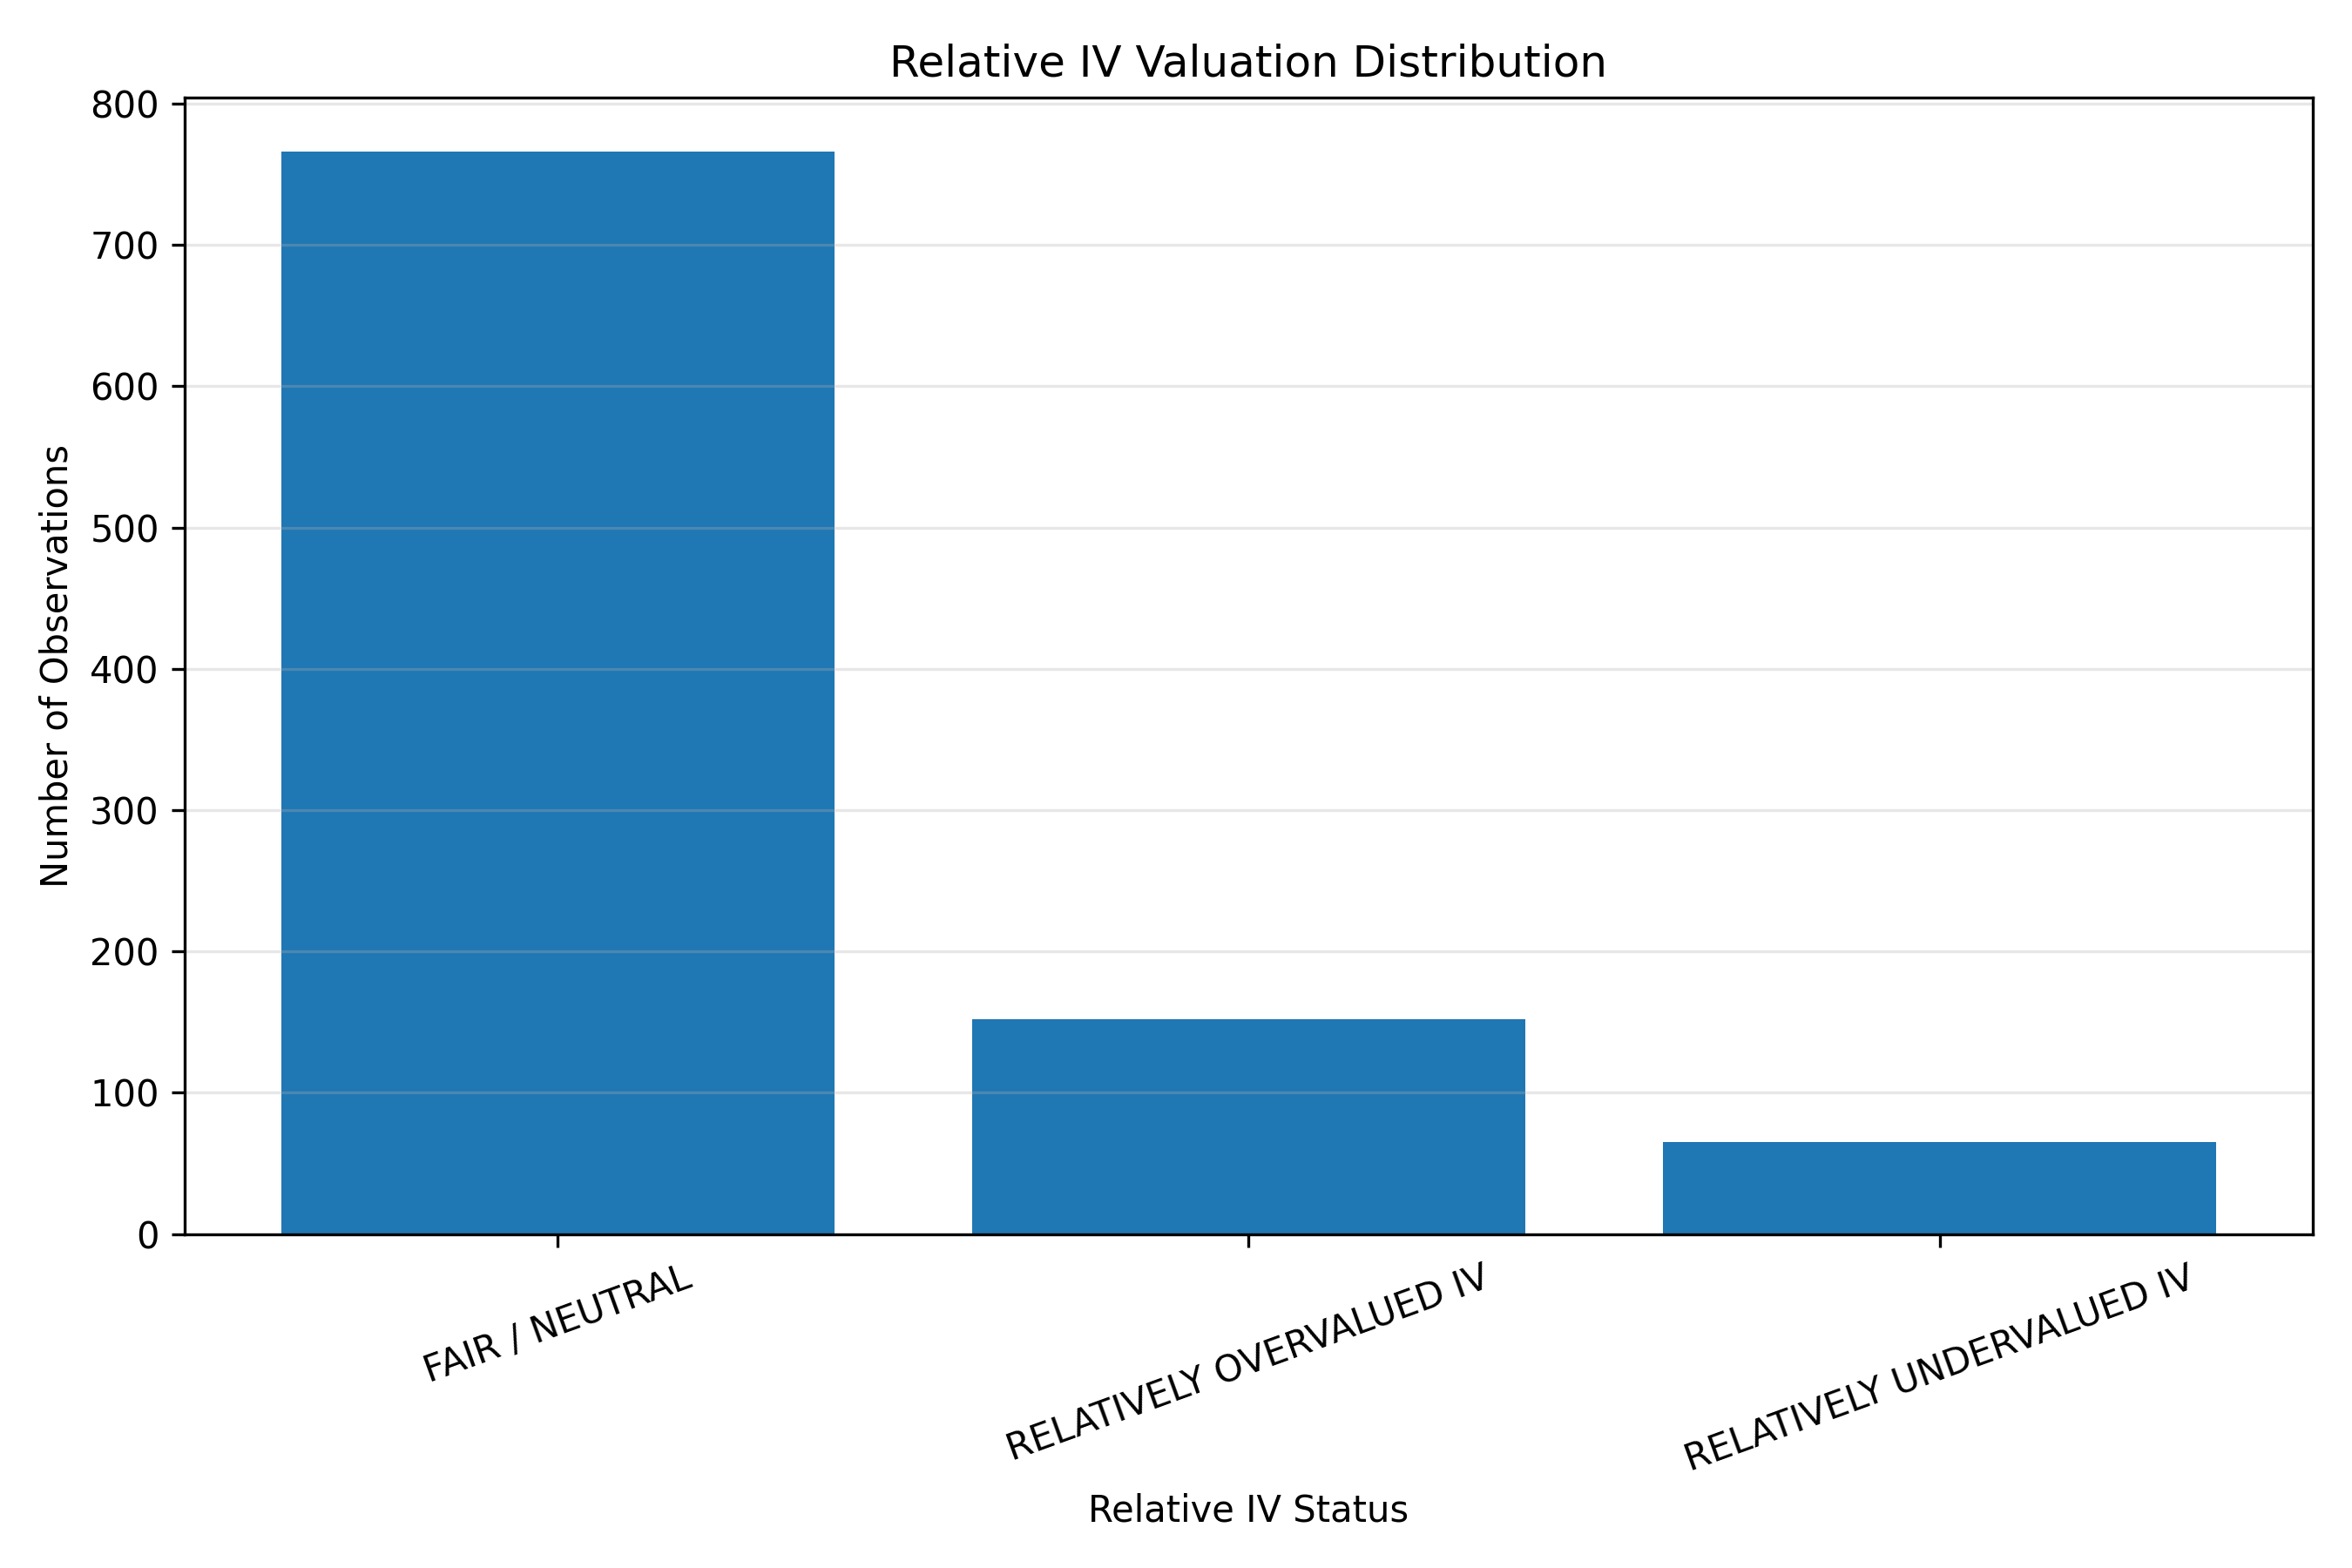
\includegraphics[width=\textwidth]{05_relative_iv_valuation_distribution.png}
        \caption{Relative Option Valuation Distribution.}
        \label{fig:relative_iv_distribution}
    \end{minipage}
    \hfill
    \begin{minipage}{0.48\textwidth}
        \centering
        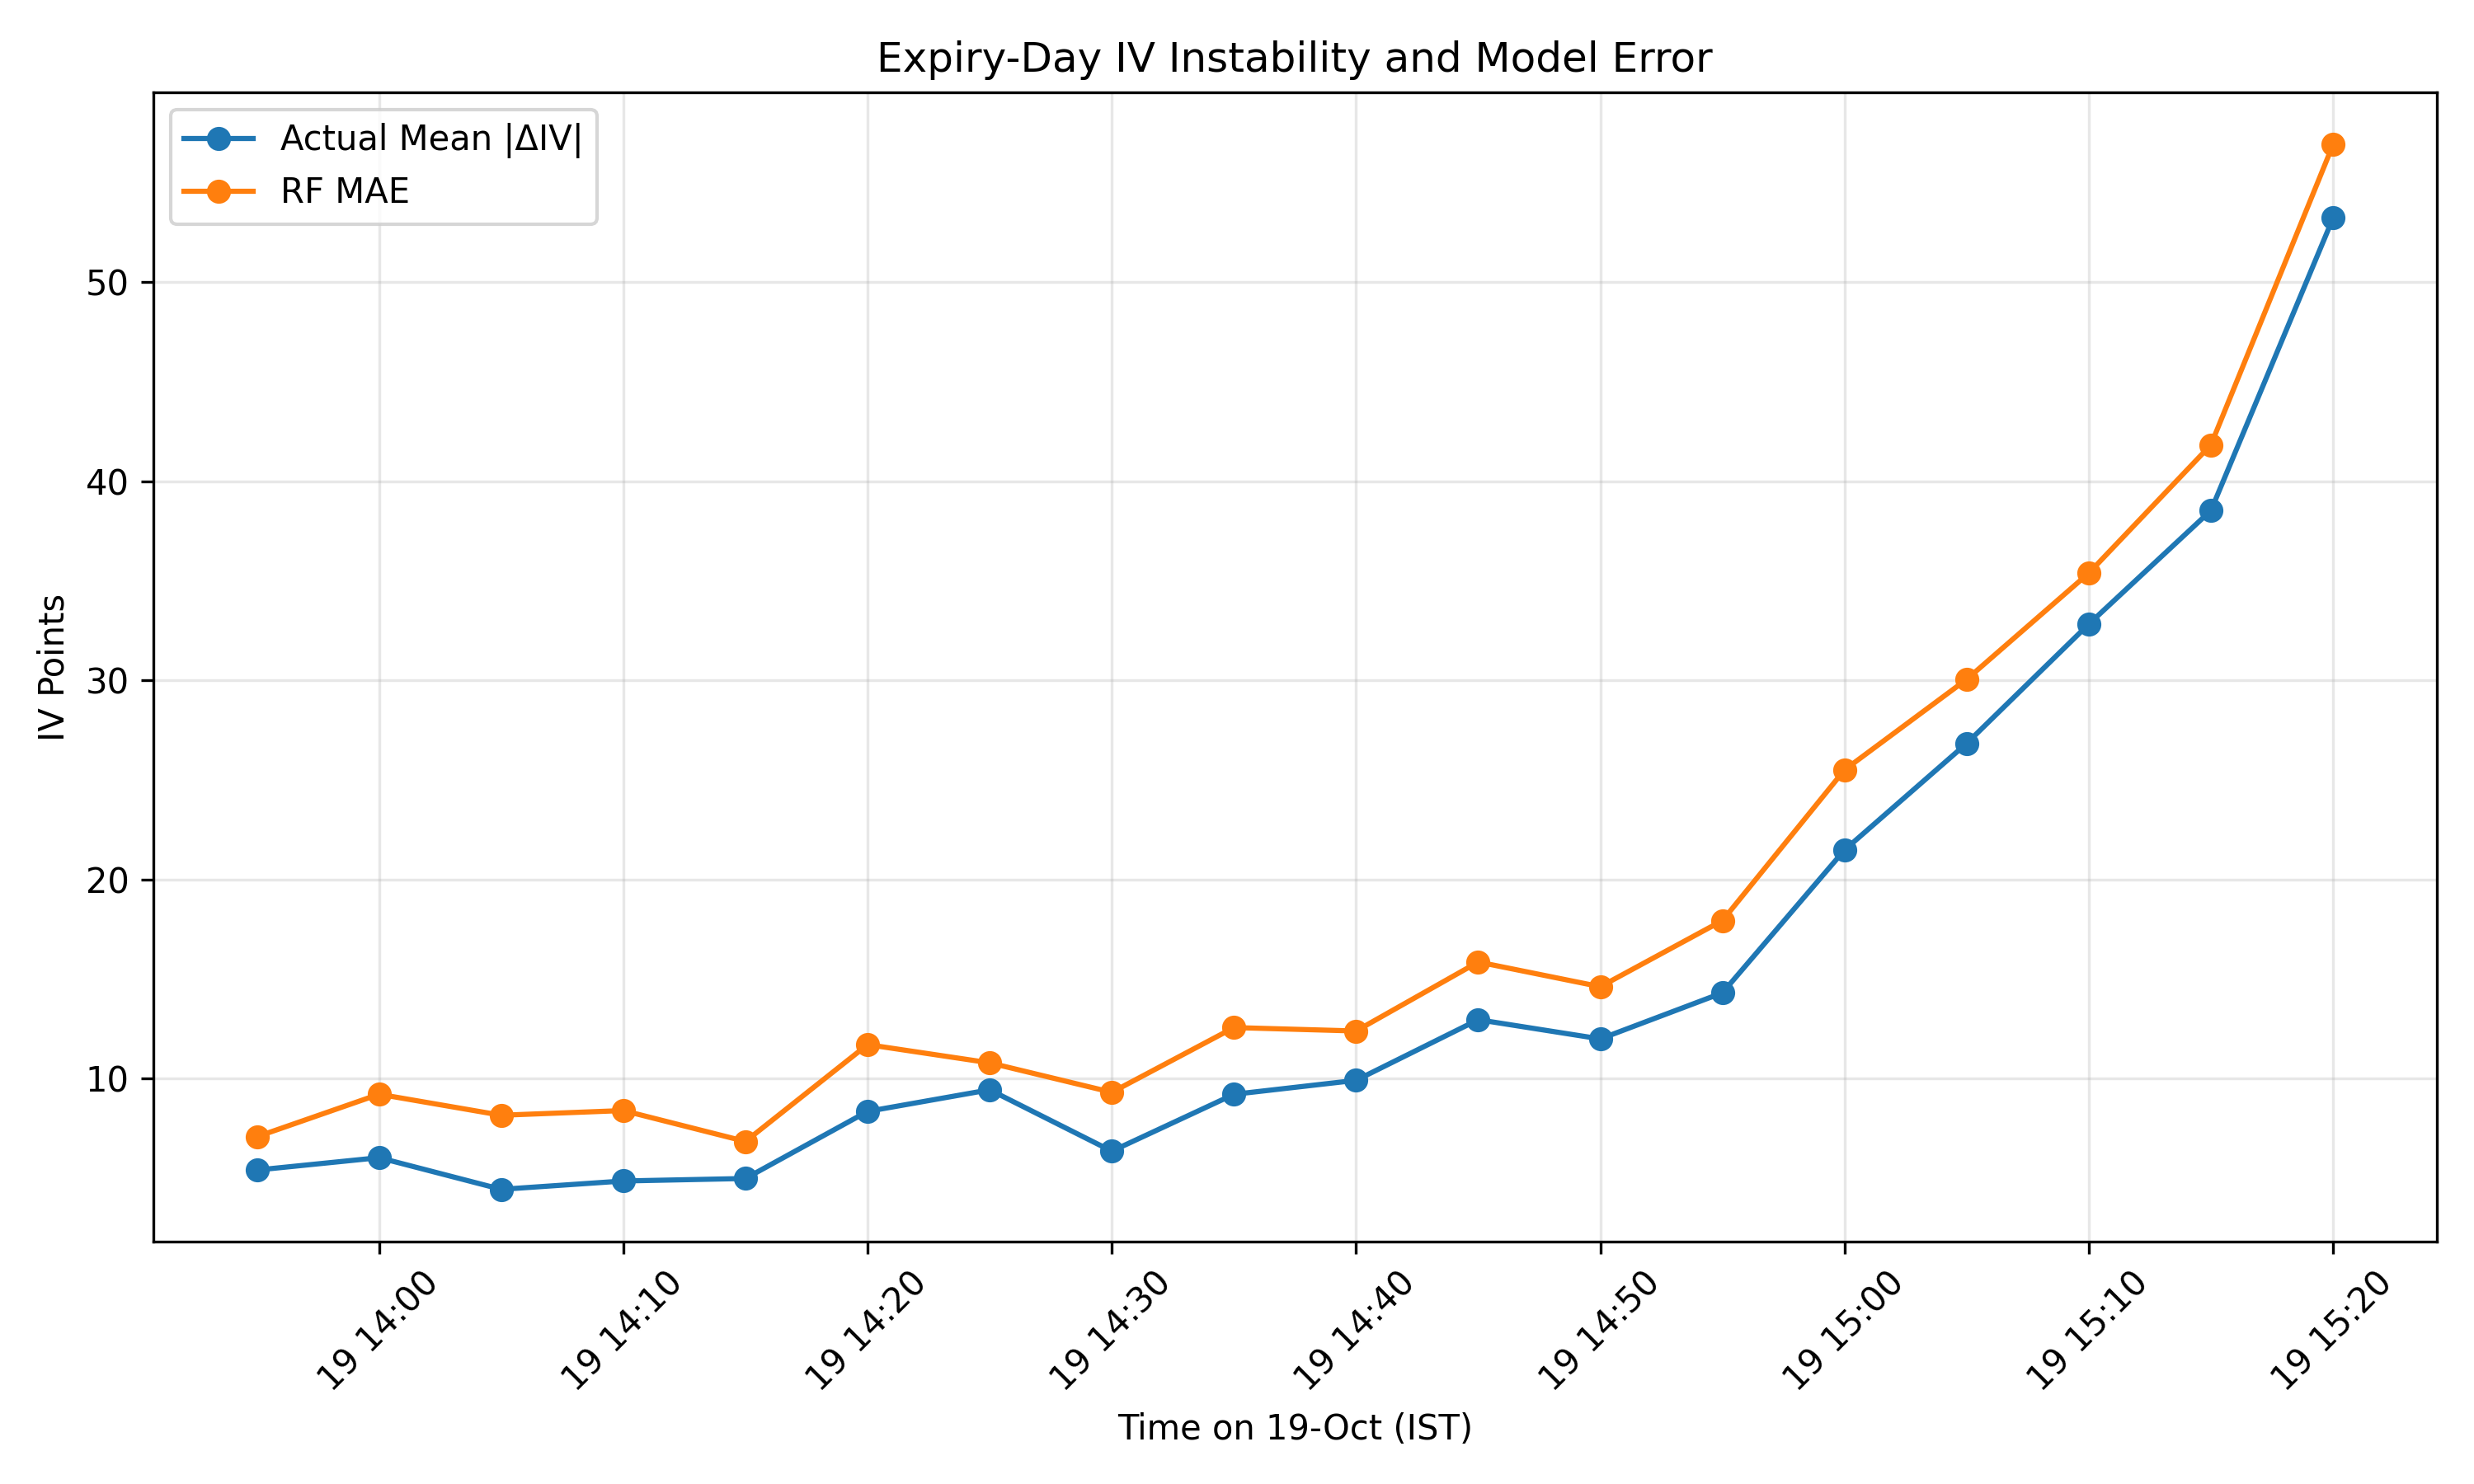
\includegraphics[width=\textwidth]{08_expiry_day_deterioration.png}
        \caption{Expiry-Day Error Spike ($<$95m TTE).}
        \label{fig:expiry_day_deterioration}
    \end{minipage}
\end{figure}

\section{Multi-Factor Scenario Stress Testing Case Study}
\label{sec:stress_testing_case_study}

To quantify non-linear derivatives risk under combined macroeconomic and market liquidity shocks, we evaluate the multi-factor Black-Scholes scenario engine.

\subsection{Case Study Contract Specification}
The analysis examines a representative near-the-money weekly call option:
\begin{itemize}
    \item \textbf{Contract Instrument:} NIFTY 50 Weekly Call Option (CE)
    \item \textbf{Strike Price ($K$):} 23,150.00 | \textbf{Underlying Spot ($S_0$):} \rupee 23,125.65 (Moneyness: 1.001)
    \item \textbf{Observed Market LTP:} \rupee 81.70 | \textbf{Current Market IV ($\sigma_0$):} 10.71\%
    \item \textbf{Time-to-Expiry ($\tau_0$):} 74.58 fractional hours (3.11 calendar days)
    \item \textbf{Theoretical BSM Base Value ($V_0$):} \textbf{\rupee 85.07}
\end{itemize}

Figures \ref{fig:spot_stress_sensitivity} and \ref{fig:iv_stress_sensitivity} present the sensitivity response curves across spot price and implied volatility shifts, respectively.

\begin{figure}[H]
    \centering
    \begin{minipage}{0.48\textwidth}
        \centering
        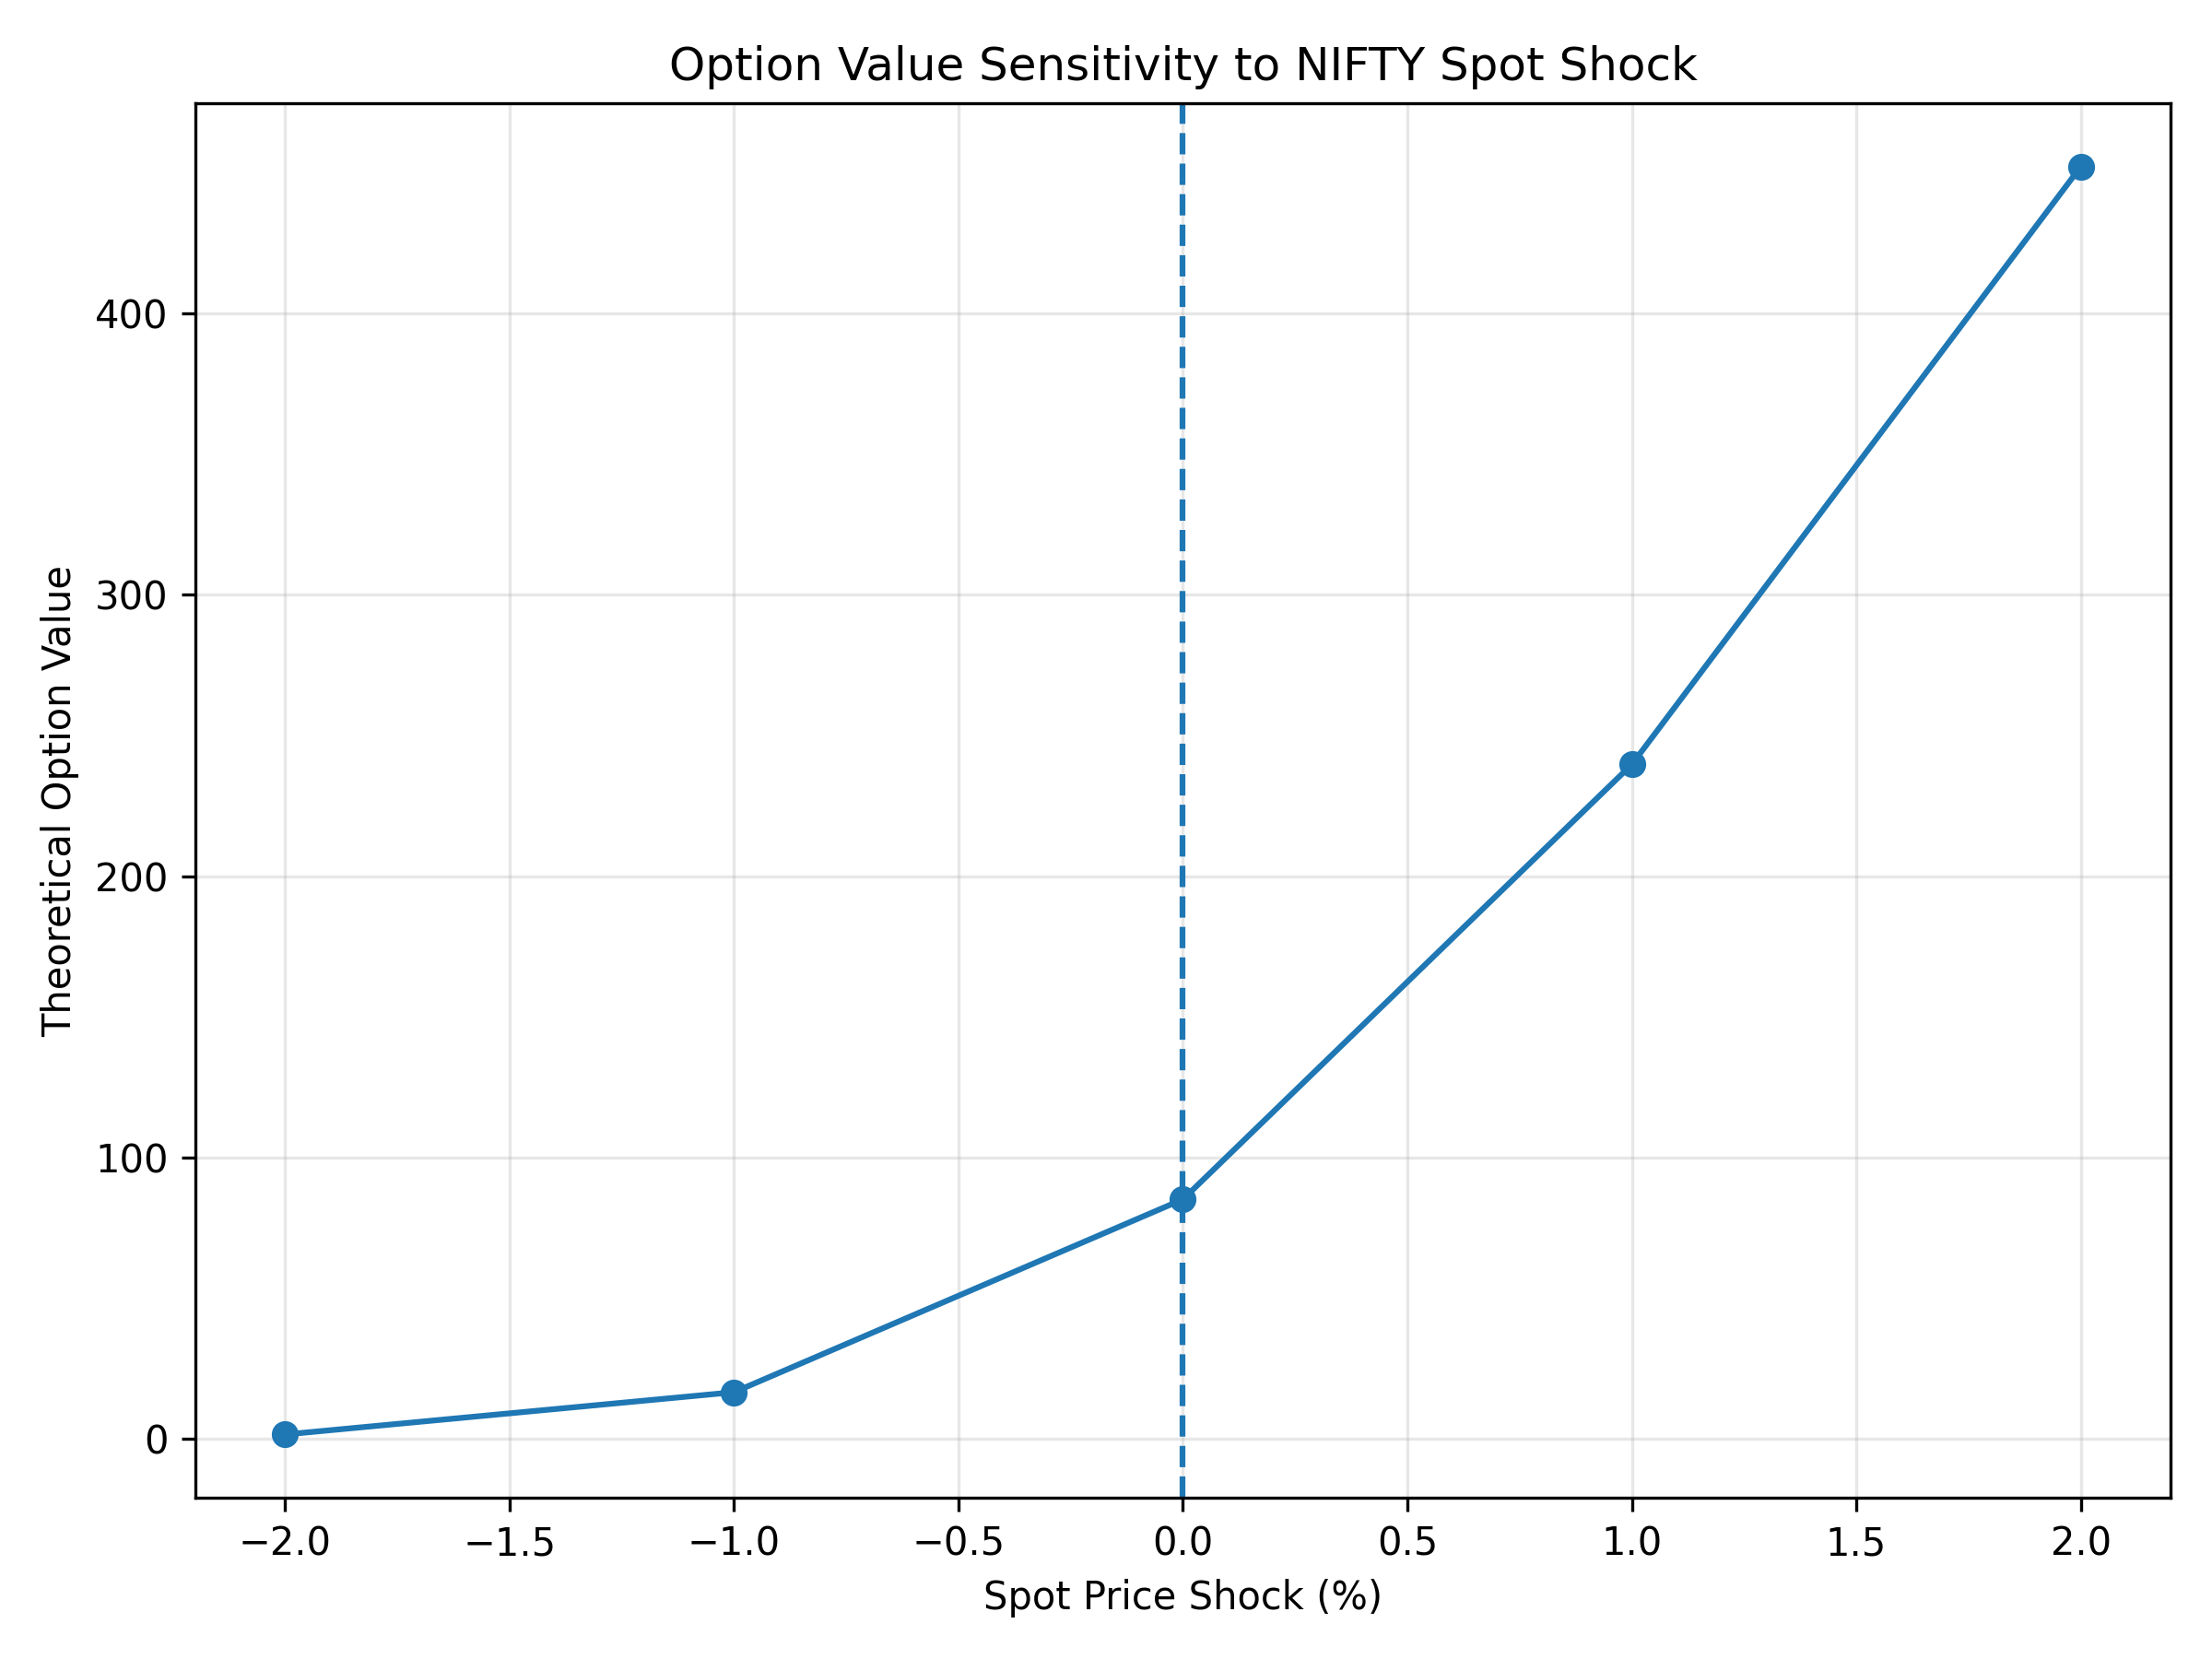
\includegraphics[width=\textwidth]{06_spot_stress_sensitivity.png}
        \caption{Option Value Sensitivity to Underlying Spot Shifts ($\pm 2\%$).}
        \label{fig:spot_stress_sensitivity}
    \end{minipage}
    \hfill
    \begin{minipage}{0.48\textwidth}
        \centering
        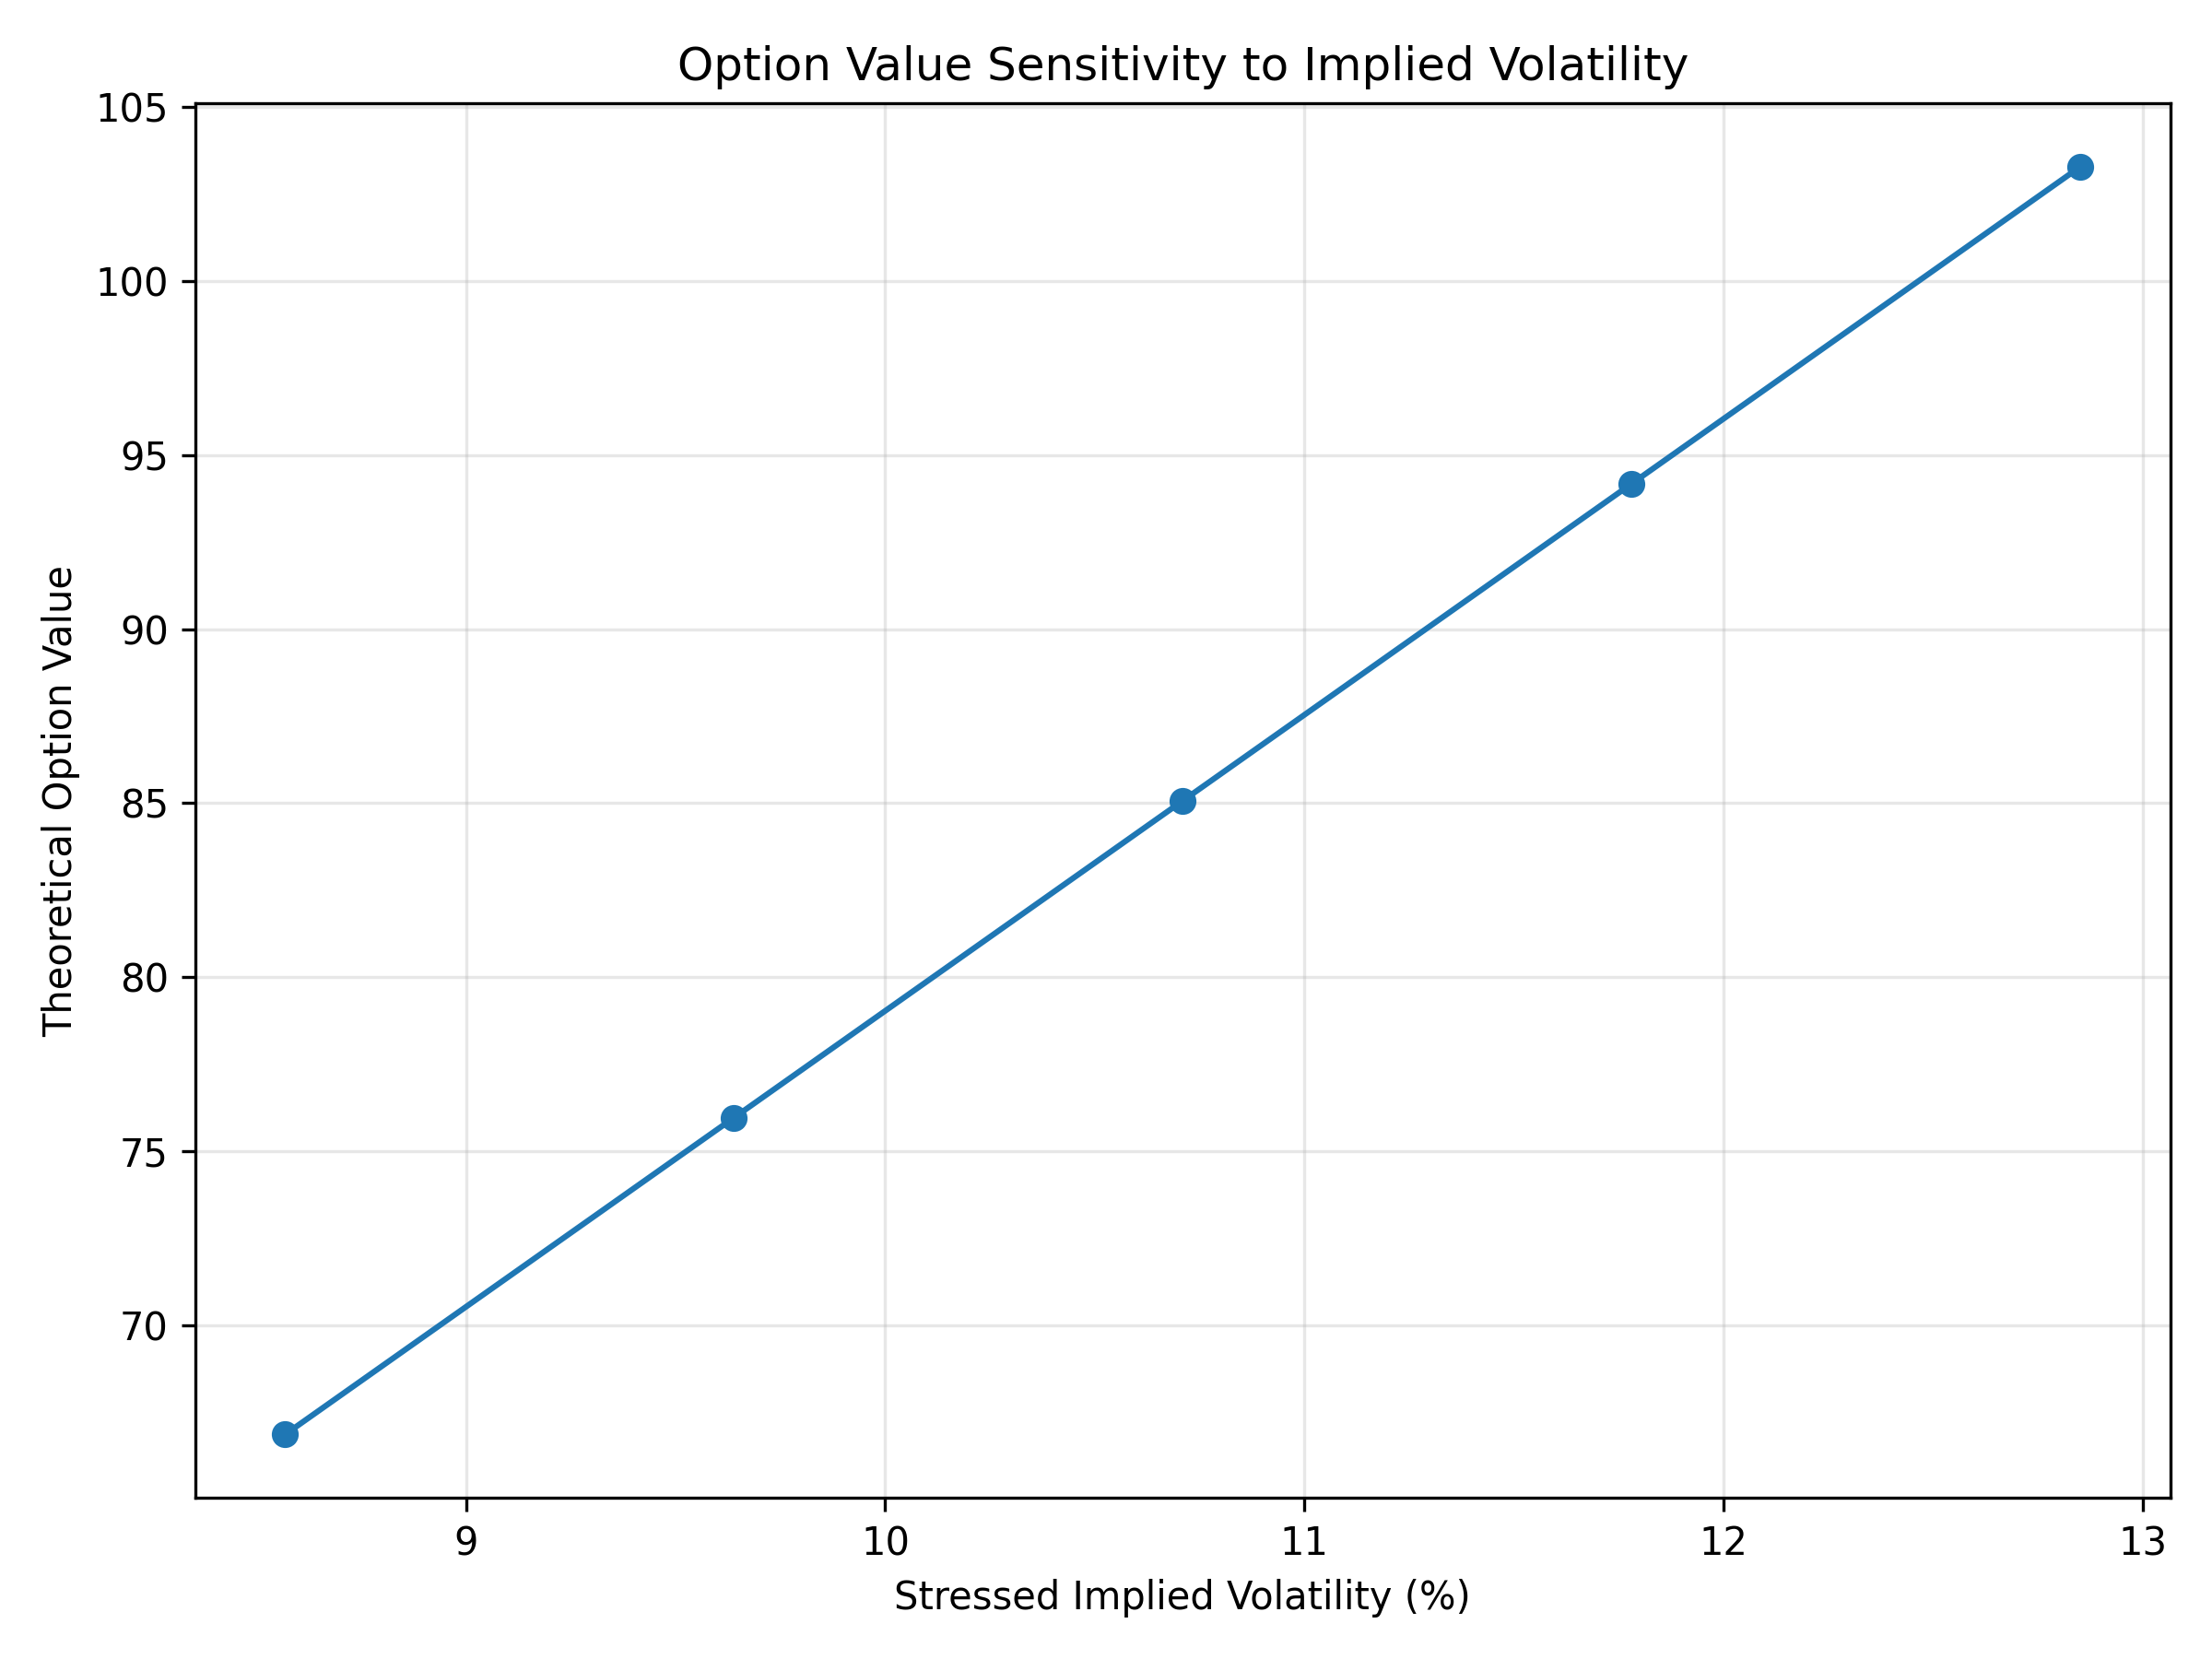
\includegraphics[width=\textwidth]{07_iv_stress_sensitivity.png}
        \caption{Option Value Sensitivity to Implied Volatility Shifts ($\pm 20\%$).}
        \label{fig:iv_stress_sensitivity}
    \end{minipage}
\end{figure}

Table \ref{tab:scenario_stress_matrix} details the complete multi-factor revaluation matrix across joint spot, volatility, and time-decay scenarios.

\begin{table}[H]
    \centering
    \footnotesize
    \caption{Multi-Factor Black-Scholes Scenario Stress Testing Matrix (NIFTY 23,150 CE).}
    \label{tab:scenario_stress_matrix}
    \begin{tabularx}{\textwidth}{lcccccr}
        \toprule
        \textbf{Scenario Description} & \textbf{Spot ($S$)} & \textbf{IV ($\sigma$)} & \textbf{TTE} & \textbf{Value} & \textbf{P\&L (\rupee)} & \textbf{P\&L (\%)} \\
        \midrule
        \textbf{Base Case} & \rupee 23,125.65 & 10.71\% & 74.58h & \textbf{\rupee 85.07} & \rupee 0.00 & \textit{0.00\%} \\
        \textbf{Moderate Bullish (+1\%)} & \rupee 23,356.91 & 10.71\% & 74.58h & \textbf{\rupee 245.70} & +\rupee 160.63 & \textbf{+188.83\%} \\
        \textbf{Moderate Bearish (-1\%)} & \rupee 22,894.39 & 10.71\% & 74.58h & \textbf{\rupee 21.85} & -\rupee 63.22 & \textbf{-74.32\%} \\
        \textbf{IV Spike (+20\% relative)} & \rupee 23,125.65 & 12.85\% & 74.58h & \textbf{\rupee 103.22} & +\rupee 18.15 & \textbf{+21.33\%} \\
        \textbf{IV Crush (-20\% relative)} & \rupee 23,125.65 & 8.57\% & 74.58h & \textbf{\rupee 66.82} & -\rupee 18.25 & \textbf{-21.46\%} \\
        \textbf{Bearish (-2\%) + IV Spike (+20\%)} & \rupee 22,663.14 & 12.85\% & 74.58h & \textbf{\rupee 4.39} & -\rupee 80.68 & \textbf{-94.84\%} \\
        \textbf{Bullish (+2\%) + IV Crush (-20\%)} & \rupee 23,588.16 & 8.57\% & 74.58h & \textbf{\rupee 450.42} & +\rupee 365.35 & \textbf{+429.47\%} \\
        \textbf{Intraday Time Decay (6h)} & \rupee 23,125.65 & 10.71\% & 68.58h & \textbf{\rupee 81.56} & -\rupee 3.51 & \textbf{-4.13\%} \\
        \textbf{Overnight Time Decay (24h)} & \rupee 23,125.65 & 10.71\% & 50.58h & \textbf{\rupee 70.04} & -\rupee 15.03 & \textbf{-17.67\%} \\
        \bottomrule
    \end{tabularx}
\end{table}

\subsection{Critical Risk Management Insights}
The multi-factor scenario matrix reveals a fundamental quantitative principle of short-dated options:
\begin{enumerate}
    \item \textbf{Delta Heavily Dominates Vega:}
    A $+1\%$ move in the underlying spot index generates a massive $+188.83\%$ surge in theoretical call value (from \rupee 85.07 to \rupee 245.70). In contrast, a massive $+20\%$ relative expansion in implied volatility (from $10.71\%$ to $12.85\%$) produces only a $+21.33\%$ gain.
    \item \textbf{The Inefficacy of Long Vega Protection in Market Crashes:}
    In Scenario 6 (a $-2\%$ spot decline combined with a $+20\%$ volatility spike), the call value plummets by **$-94.84\%$** (collapsing to \rupee 4.39). Even though implied volatility expanded dramatically, the positive vega P\&L was completely overwhelmed by catastrophic negative delta losses.
    \item \textbf{Operational Takeaway:} Trading desks cannot trade volatility in isolation. High-frequency implied volatility forecasts must always be coupled with dynamic delta hedging to neutralize underlying price risk.
\end{enumerate}

\section{The Expiry-Day Structural Regime Breakdown (October 19 Forensic Experiment)}
\label{sec:expiry_day_breakdown}

A cornerstone academic contribution of this thesis is the empirical discovery and econometric diagnosis of the **Expiry-Day Structural Regime Shift**.

To test the operational robustness of the trained Random Forest model under out-of-sample stress, the model was deployed on an unseen dataset collected on **October 19, 2026**—an active weekly options expiry session.
\begin{itemize}
    \item \textbf{Training Regime ($T_{\text{train}}$):} October 15--16, 2026; Time-to-Expiry ranged between **74.6 and 100.6 hours**.
    \item \textbf{Testing Regime ($T_{\text{expiry}}$):} October 19, 2026; Time-to-Expiry collapsed to between **0.17 and 1.58 hours** (10 minutes to 95 minutes prior to contract settlement).
\end{itemize}

Figure \ref{fig:expiry_day_deterioration} (paired in Section \ref{sec:relative_valuation_results}) illustrates the chronological trajectory of prediction errors as trading approached the final closing bell.

Table \ref{tab:expiry_day_collapse_metrics} compares model performance between the normal mid-week development regime and the October 19 expiry-day regime.

\begin{table}[H]
    \centering
    \footnotesize
    \caption{Empirical Breakdown Metrics: Development Test Set vs. October 19 Expiry Day.}
    \label{tab:expiry_day_collapse_metrics}
    \begin{tabularx}{\textwidth}{p{3.8cm}ccX}
        \toprule
        \textbf{Metric} & \textbf{Development (74--100h TTE)} & \textbf{Expiry-Day ($<$1.58h TTE)} & \textbf{Performance Impact} \\
        \midrule
        \textbf{Time-to-Expiry Horizon} & 74.6 to 100.6 hours & 0.17 to 1.58 hours & 98.4\% maturity contraction \\
        \textbf{Random Forest MAE} & \textbf{0.5214 pts} & \textbf{17.42 pts} & \textbf{3,241\% Error Explosion} \\
        \textbf{Persistence Baseline MAE} & \textbf{0.5505 pts} & \textbf{14.47 pts} & Outperformed ML by 2.95 pts \\
        \textbf{Directional Hit-Rate} & \textbf{53.20\% (63.4\% at $\theta=0.1$)} & \textbf{19.09\%} & Severe Inversion (Sub-Random) \\
        \textbf{Maximum Single Error} & 3.42 pts & 148.60 pts & Extreme tail divergence \\
        \bottomrule
    \end{tabularx}
\end{table}

\subsection{Econometric \& Mathematical Diagnosis of the Breakdown}
The catastrophic breakdown observed in Table \ref{tab:expiry_day_collapse_metrics} confirms Hypothesis 4 ($H_4$). A forensic investigation reveals four distinct mathematical and structural mechanisms driving this failure:

\begin{enumerate}
    \item \textbf{Hyperbolic Gamma and Theta Singularity as $\tau \to 0$:}
    As derived in Section \ref{subsec:gamma_derivation} and \ref{subsec:theta_derivation}:
    \begin{equation}
        \lim_{\tau \to 0} \Gamma_{\text{ATM}} = +\infty, \quad \lim_{\tau \to 0} \Theta_{\text{ATM}} = -\infty
    \end{equation}
    In the final 90 minutes before settlement, an option's extrinsic time value vanishes vertically. Any minor tick in the NIFTY 50 spot index causes immediate, discontinuous flips between pure intrinsic value and total worthlessness. The continuous diffusion assumptions underpinning mid-week volatility dynamics are mathematically violated.

    \item \textbf{The Vanishing Vega Breakdown:}
    As derived in Section \ref{subsec:vega_derivation}:
    \begin{equation}
        \lim_{\tau \to 0} \nu = \lim_{\tau \to 0} S \sqrt{\tau} N'(d_1) = 0
    \end{equation}
    Because Vega drops to near-zero ($10^{-5}$), option market prices cease to respond to volatility changes. In the Newton-Raphson inversion algorithm (Equation \eqref{eq:newton_raphson_iv}):
    \begin{equation}
        \Delta \sigma = -\frac{\Delta C}{\nu} \implies \lim_{\nu \to 0} \left| \frac{\Delta C}{\nu} \right| = \infty
    \end{equation}
    A tiny exchange reporting anomaly of \rupee 0.10 causes the inverted implied volatility quote to explode by 100 to 200 percentage points, creating extreme artificial volatility spikes.

    \item \textbf{Severe Covariate Shift (Out-of-Distribution Feature Space):}
    The Random Forest model was trained on observations where \texttt{exact\_tte\_hours} $\in [74.6, 100.6]$. On expiry afternoon, the feature values collapsed to $[0.17, 1.58]$. Tree-based models cannot extrapolate beyond the minimum and maximum feature thresholds observed during training. When presented with completely out-of-distribution temporal inputs, the decision tree split nodes traverse to arbitrary terminal leaves, generating erratic, uncalibrated forecasts.

    \item \textbf{Microstructure Discontinuity \& Institutional Pin Risk:}
    Between 14:00 and 15:30 IST on weekly expiry days, institutional market makers aggressively square off large inventory positions, roll open interest into the subsequent weekly cycle, and manage pin risk around strike boundaries. Order books become thin, bid-ask spreads widen erratically, and quotes jump discretely rather than diffusing smoothly.
\end{enumerate}

\subsection{Core Academic Conclusion for Quantitative Trading}
This empirical finding proves that **a single static machine learning model cannot be deployed across all phases of the options contract lifecycle**. Institutional trading systems must implement a **Regime-Switching Architecture**:
\begin{itemize}
    \item \textit{Regime 1 (Standard Non-Expiry Model):} Active when $\text{TTE} \ge 6.0\text{ hours}$. Utilizes the trained Random Forest ensemble with autoregressive momentum lags.
    \item \textit{Regime 2 (Expiry-Day Sub-2-Hour Model):} Active when $\text{TTE} < 2.0\text{ hours}$. Suspends continuous IV forecasting, disables vega-based relative valuation, and transitions execution to gamma-hedging, parity arbitrage, and discrete order-flow jump models.
\end{itemize}
